\documentclass[oneside, colophon, english]{phduio}
\usepackage{phdstyle}
\usepackage{amsfonts,amsmath,mathtools}
\usepackage{bm}
\usepackage{listings, enumerate}
\usepackage{float}
\usepackage{xcolor}
\usepackage{pgfplots, pgf, tikz}
\usetikzlibrary{arrows,automata}
%\usepgfplotslibrary{colormaps}
\definecolor{RED}{HTML}{EB6231}
\definecolor{YELLOW}{HTML}{E29D26}
\definecolor{BLUE}{HTML}{5D80B4}
\definecolor{LIGHTGREEN}{HTML}{6ABD9B}
\definecolor{GREEN}{HTML}{8FB03E}
\definecolor{PURPLE}{HTML}{BE1E2D}
\definecolor{BROWN}{HTML}{A97C50}
\definecolor{PINK}{HTML}{DA1C5C}
\pgfplotsset{every axis/.append style={line width=1pt}}
\pgfplotscreateplotcyclelist{colors}{RED\\YELLOW\\BLUE\\LIGHTGREEN\\GREEN\\}

\usepackage[toc]{glossaries}
\makeglossaries
\definecolor{RED}{HTML}{EB6231}
\definecolor{YELLOW}{HTML}{E29D26}
\definecolor{BLUE}{HTML}{5D80B4}
\definecolor{LIGHTGREEN}{HTML}{6ABD9B}
\definecolor{GREEN}{HTML}{8FB03E}
\definecolor{PURPLE}{HTML}{BE1E2D}
\definecolor{BROWN}{HTML}{A97C50}
\definecolor{PINK}{HTML}{DA1C5C}

\newcommand{\der}{\mathrm{d}}
\newcommand{\e}{\mathrm{e}}
\newcommand{\dnds}{dNdS}
\newcommand{\indice}{l}
\newcommand{\indiceexp}{^{(\indice)}}
% Time, effective population size and mutation rate.
\newcommand{\Ne}{N}
% \acrshort{DNA}
\newcommand{\SetNuc}{\Omega_{\mathrm{N}}}
\newcommand{\SetWeak}{\Omega_{\mathrm{W}}}
\newcommand{\SetStrong}{\Omega_{\mathrm{S}}}
\newcommand{\mutmatrix}{R}
\newcommand{\Mutmatrix}{\bm{\mutmatrix}_{4\times4}}
\newcommand{\exchan}{\rho}
\newcommand{\Exchan}{\bm{\exchan}_{6\times1}}
\newcommand{\mutequi}{\sigma}
\newcommand{\Mutequi}{\bm{\mutequi}_{4\times1}}
% Codons
\newcommand{\SetCodon}{\Omega_{\mathrm{C}}}
\newcommand{\ci}{{i}}
\newcommand{\cj}{{j}}
\newcommand{\itoj}{\ci, \cj}
\newcommand{\nucitoj}{\mathcal{M}(\itoj)}
\newcommand{\submatrix}{Q}
\newcommand{\Submatrix}{\bm{\submatrix}_{61\times61}}
\newcommand{\subequi}{\pi}
\newcommand{\Subequi}{\bm{\subequi}_{61\times1}}
\newcommand{\probmatrix}{P}
\newcommand{\Probmatrix}{\bm{\probmatrix}_{61\times61}}
% Amino-acids
\newcommand{\SetAa}{\Omega_{\mathrm{A}}}
\newcommand{\Neighbor}{\mathcal{V}}
\newcommand{\NonSyn}{\mathcal{N}}
\newcommand{\Syn}{\mathcal{S}}
\newcommand{\Nx}{\Neighbor_x}
\newcommand{\NxAB}{\Neighbor_x^{\mathrm{A} \rightarrow \mathrm{B}}}
\newcommand{\NyBA}{\Neighbor_x^{\mathrm{B} \rightarrow \mathrm{A}}}
\newcommand{\NxWS}{\Neighbor_x^{\mathrm{W} \rightarrow \mathrm{S}}}
\newcommand{\NxSS}{\Neighbor_x^{\mathrm{S} \rightarrow \mathrm{S}}}
\newcommand{\NxSW}{\Neighbor_x^{\mathrm{S} \rightarrow \mathrm{W}}}
\newcommand{\NxWW}{\Neighbor_x^{\mathrm{W} \rightarrow \mathrm{W}}}
\newcommand{\NyWS}{\Neighbor_y^{\mathrm{W} \rightarrow \mathrm{S}}}
\newcommand{\NySS}{\Neighbor_y^{\mathrm{S} \rightarrow \mathrm{S}}}
\newcommand{\NySW}{\Neighbor_y^{\mathrm{S} \rightarrow \mathrm{W}}}
\newcommand{\NyWW}{\Neighbor_y^{\mathrm{W} \rightarrow \mathrm{W}}}
\newcommand{\NxNonSyn}{\NonSyn_x}
\newcommand{\NyNonSyn}{\NonSyn_y}
\newcommand{\NxSyn}{\Syn_x}
\newcommand{\NySyn}{\Syn_y}
\newcommand{\aminoacid}{\text{A}}
\newcommand{\aai}{\mathcal{A}(\ci)}
\newcommand{\aaj}{\mathcal{A}(\cj)}
\newcommand{\Ni}{\mathcal{N}_{\mathrm{eighbors}}\left(\ci\right)}
\newcommand{\NiNonSyn}{\mathcal{N}_{\mathrm{onSyn}}\left(\ci\right)}
\newcommand{\NiSyn}{\mathcal{S}_{\mathrm{yn}}\left(\ci\right)}
\newcommand{\fit}{f}
\newcommand{\Fit}{\bm{\fit}_{20\times1}}
\newcommand{\fiti}{\fit_{\aai}}
\newcommand{\fitj}{\fit_{\aaj}}
\newcommand{\scaledfit}{F}
\newcommand{\ScaledFit}{\bm{\scaledfit}_{20\times1}}
\newcommand{\scaledfiti}{\scaledfit_{\aai}}
\newcommand{\scaledfitj}{\scaledfit_{\aaj}}
\newcommand{\selcoef}{{\delta_{\fit}}}
\newcommand{\scaledselcoef}{{\Delta \scaledfit}}
% Tree
\newcommand{\Tree}{\mathcal{T}}
\newcommand{\node}{\text{v}}
\newcommand{\taxon}{\node}
\newcommand{\Settaxon}{1 \leq \taxon \leq \Ntaxa}
\newcommand{\Ntaxa}{P}
\newcommand{\treeroot}{0}
\newcommand{\treerootexp}{^{(\treeroot)}}
\newcommand{\branch}{\text{w}}
\newcommand{\branchexp}{^{(\branch)}}
\newcommand{\Nbranch}{2 \Ntaxa - 2}
\newcommand{\Setbranch}{1 \leq \branch \leq 2 \Ntaxa - 2}
\newcommand{\up}{\branch^{\uparrow}}
\newcommand{\down}{\node}
\newcommand{\nodeexp}{^{(\node)}}
\newcommand{\Nnode}{2 \Ntaxa - 2}
\newcommand{\Ninternal}{\Ntaxa - 2}
\newcommand{\Setnode}{\treeroot \leq \node \leq 2 \Ntaxa - 2}
\newcommand{\Setnodenoroot}{1 \leq \node \leq 2 \Ntaxa - 2}
\newcommand{\Setinternal}{\Ntaxa + 1 \leq \node \leq 2 \Ntaxa - 2}
\newcommand{\branchnode}{\mathcal{W}}
\newcommand{\age}{T}
\newcommand{\branchtime}{\Delta \age}
\newcommand{\branchlength}{L}
% Alignment
\newcommand{\data}{{\color{PINK}{D}}}
\newcommand{\Data}{\bm{\data}}
\newcommand{\site}{\text{s}}
\newcommand{\siteexp}{^{(\site)}}
\newcommand{\Nsite}{\text{N}_{\site}}
\newcommand{\Setsite}{1 \leq \site \leq \Nsite}
\newcommand{\branchsiteexp}{^{(\branch, \site)}}
\newcommand{\treerootsiteexp}{^{(\treeroot, \site)}}
\newcommand{\taxonsiteexp}{^{(\taxon, \site)}}
% Categories
\newcommand{\cat}{\text{k}}
\newcommand{\catVar}{\mathcal{K}}
\newcommand{\catexp}{^{(\cat)}}
\newcommand{\Ncat}{\text{N}_{\cat}}
\newcommand{\Setcat}{1 \leq \cat \leq \Ncat}
\newcommand{\catsite}{\catVar^{\left(\site\right)}}
\newcommand{\branchcatexp}{^{(\branch, \cat)}}
\newcommand{\treerootcatexp}{^{(\treeroot, \cat)}}
% Polymorphism
\newcommand{\copies}{\text{n}}
\newcommand{\samples}{\text{N}_{\copies}}
% Random variables
\newcommand{\pruning}{\psi}
\newcommand{\uniform}{0, 1}
\newcommand{\Identitymatrix}{\bm{I}_{2\times2}}
\newcommand{\brownian}{\bm{B}_{2\times1}}
\newcommand{\contrast}{\bm{C}_{2\times1}}
\newcommand{\Covariancematrix}{\bm{\varSigma}_{2\times2}}
\newcommand{\covariancedf}{q}
\newcommand{\covariancekappa}{\kappa}
\newcommand{\Scattermatrix}{\bm{A}_{2\times2}}
\newcommand{\Multivariate}{\bm{Z}_{2\times1}}
\newcommand{\base}{\varPi}
\newcommand{\Base}{\bm{\base}_{20\times1}}
\newcommand{\baseconc}{\alpha}
\newcommand{\Basecenter}{\bm{\gamma}_{20\times1}}
\newcommand{\stickbreaking}{\varOmega}
\newcommand{\StickBreaking}{\bm{\stickbreaking}_{\Ncat\times1}}
\newcommand{\stick}{\varPhi}
\newcommand{\stickbreakinghyper}{\beta}
% Mapping
\newcommand{\history}{\mathcal{H}}
\newcommand{\sn}{{\color{BLUE}{S}}}
\newcommand{\s}{{\color{LIGHTGREEN}{S_0^{k}}}}
\newcommand{\si}{{\color{PINK}{S_1^{k}}}}
\newcommand{\sii}{{\color{PINK}{S_2^{k}}}}
\newcommand{\siii}{{\color{PINK}{S_3^{k}}}}
\newcommand{\siiii}{{\color{PINK}{S_4^{k}}}}
\newcommand{\siiiii}{{\color{LIGHTGREEN}{S_5^{k}}}}


\renewcommand{\contentsname}{Table of contents}
\author{Thibault Latrille}
\title{}
\department{}
\affiliation{Université de Lyon \and ENS de Lyon}

\includeonly
{	
	sections/frontpage,
    sections/dedication,
    sections/abstract,
    sections/abstract_fr,
    sections/acknowledgement,
    sections/notations,
    sections/preamble,
    sections/papers,
    sections/introduction,
    sections/paperI,
    sections/paperII,
    sections/paperIII,
    sections/discussion,
    sections/conclusion,
    sections/appendixA,
}

\begin{document}

	\frontmatter        % Folios in Roman numerals, unnumbered chapters.
	
	\thispagestyle{empty}
\vspace*{\stretch{1}}

\unitlength 1cm
\begin{center}

    \vspace*{-2.5cm}
    \begin{figure}[h]
        \centering
        
\includegraphics[width=0.8\textwidth]{figures/logo-UdL-UCB}
    \end{figure}

    {\large \textbf{THÈSE de DOCTORAT DE L'UNIVERSITÉ DE LYON}\\}
    {Opérée au sein de~:\\}
    {\large \textbf{l'Université Claude Bernard Lyon 1}\\}
    \vspace{12pt}
    {\large \textbf{Ecole Doctorale} 341 \\
    \vspace{0.15cm}
    Écosystèmes Évolution Modélisation Microbiologie
    }
    
    \vspace{12pt}

    {\large \textbf{Spécialité de doctorat~:} Génomique évolutive
    \\}

    \vspace{0.8cm}

    %{Soutenue publiquement le jj/mm/aaaa, par~:\\}
    {Soutenance prévue le 30/11/2020, par~:\\}
    \vspace{0.15cm}
    {\Large \textbf{Thibault Latrille}}
    \vspace{0.5cm}

    \rule{5cm}{1pt}
    \vspace{12pt}

    {\huge \textbf{Modélisation de l'articulation des mécanismes adaptatifs et neutres dans l’évolution des séquences d’ADN codant pour des protéines.}\par}

    \vspace{12pt}
    \rule{5cm}{1pt}

    \vspace{0.5cm}

\end{center}

Devant le jury composé de~:\\

\small {
\begin{tabular}{ll}
    \textbf{Celine BROCHIER-ARMANET} & \textbf{Présidente}         \\
    Professeure, Université Claude Bernard Lyon 1 \\
    \textbf{Julien Yann DUTHEIL}     & \textbf{Rapporteur}         \\
    Research Group Leader, Max Planck Institute (Allemagne) \\
    \textbf{Richard GOLDSTEIN}       & \textbf{Rapporteur}         \\
    Professeur, University College London (Royaume-Uni) \\
    \textbf{Carina Farah MUGAL}      & \textbf{Rapporteure}        \\
    Chercheure, Uppsala University (Suède) \\
    \textbf{Nicolas LARTILLOT}       & \textbf{Directeur de thèse} \\
    Directeur de recherche, CNRS/LBBE \\
\end{tabular}
}
\vspace*{\stretch{3}}
    \thispagestyle{empty}
\vspace*{\stretch{1}}
\begin{flushright}
    \emph{L'humanité est constamment aux prises avec deux processus contradictoires dont l'un tend à instaurer l'unification, tandis que l'autre vise à maintenir ou à rétablir la diversification.}\\
    Claude Lévi-Strauss.\\
    
    \rule{5cm}{1pt}
    
%    \emph{Humanity is constantly grappling with two contradictory processes, one of which tends to establish unification, while the other aims to maintain or restore diversification.}\\
%    Claude Lévi-Strauss, anthropologist and ethnologist, 1908-2009.
\end{flushright}
\vspace*{\stretch{3}}
    \begin{center}
	\LARGE
	\textbf{Modeling the articulation of adaptive and neutral mechanisms in the evolution of protein coding DNA sequences}
\end{center}

\section*{Abstract}

Molecular evolution aims to characterize the mechanisms at work in the evolution of sequences.
Sequences evolution is thus governed by a stochastic process composed of a mutation, selection and genetic drift.
In the long term, this stochastic process results in a history of substitution events along species trees, inducing complex patterns of molecular divergence between species.
By analysing them, phylogenetic codon models aim at capturing the intrinsic parameters of evolution.
In this context, this thesis has been focused on phylogenetic codon models, and on modelling the interplay between mutation, selection and drift shaping protein-coding DNA sequences.
Because the composition of protein coding DNA sequences does not reflect the underlying mutational process, but its filtering by selection at the level of amino acids, a careful modeling is necessary to tease apart mutation and selection.
Therefore, I first developed a phylogenetic codon model of inference in which different rates of evolution gives an accurate representation of how mutation and selection oppose each other at equilibrium.
Between the opposing forces of mutation and selection, the balance is arbitrated by genetic drift, which in turn is modulated by effective population size ($\Ne$).
As a consequence, variation of $\Ne$ along of a phylogeny can theoretically be inferred from the trails of substitutions along the lineages.
I thus developed a second model of inference, reconstructing altogether site-specific fitness landscape, long-term trends in $\Ne$ and in the mutation rate along the phylogeny.
This bayesian framework was tested against simulated data and then applied to empirical data.
Estimates of the variation of $\Ne$ corresponds to the expected direction of correlation with life-history traits or ecological variables.
However, the magnitude of inferred variation is narrower than expected.
Such as to understand this effect, I finally developed a theoretical model describing how changes in both $\Ne$ or expression level or protein will translate in change in the rate substitution, under the assumption that protein are selected against misfolding.
It is building block to bridge phylogeny and population-genetics, constructing an integrated framework is theoretically possible but with limited scope.

    \thispagestyle{empty}

\section*{Résumé}

L'évolution moléculaire vise à caractériser les mécanismes à l'œuvre dans l'évolution des séquences, régie par un processus stochastique dont les principaux composants sont la mutation, la sélection et la dérive génétique.
À long terme, ce processus stochastique se traduit par une histoire d'événements de substitutions le long des arbres d'espèces, induisant des motifs complexes de divergence moléculaire entre les espèces.
En analysant ces divergences, les modèles de codons phylogénétiques visent à capturer les paramètres intrinsèques de l'évolution.
Dans ce contexte, cette thèse s'est concentrée sur les modèles à codons phylogénétiques et sur la modélisation de l'interaction entre la mutation, la sélection et la dérive génétique dans les séquences d'ADN codant pour des protéines.
Parce que la composition de ces séquences ne reflète pas le processus de mutation sous-jacent, mais son filtrage par sélection au niveau des acides aminés, une modélisation minutieuse est nécessaire pour démêler la mutation et la sélection.
Ainsi, j'ai développé un modèle d'inférence phylogénétique dans lequel différents taux d'évolution donnent une représentation précise de la manière dont la mutation et la sélection s'opposent à l’équilibre.
Deuxièmement, l'équilibre entre mutation et sélection est arbitré par la dérive génétique, qui est médiée par la taille efficace de la population, et ses changements le long d'une phylogénie peuvent être déduits des motifs de substitutions le long des lignées.
J'ai ainsi développé un deuxième modèle d'inférence, reconstituant à la fois le paysage de fitness en chaque site, les tendances à long terme de taille efficace de population et les changements de taux de mutation le long de la phylogénie.
Ce cadre bayésien a été testé sur des données simulées puis appliqué à des données empiriques.
Les estimations de la variation de taille efficace de population correspondent à la direction attendue de la corrélation avec les traits d’histoire de vie ou les variables écologiques, bien que l'ampleur de la variation de la taille efficace de population estimée soit étroite.
Afin de comprendre cette variation étroite de la taille efficace de population estimée, j'ai finalement développé un modèle théorique décrivant comment les changements à la fois de taille efficace de population ou du niveau d'expression ou la protéine se traduisent par un changement du taux de substitution, sous l'hypothèse que les protéines sont sous sélection directionnelle pour maximiser leur stabilité conformationnelle.
Cette réponse est déterminée en fonction des paramètres moléculaires de la biophysique des protéines, et implique une faible réponse du taux de substitution aux changements de niveau d'expression ou de taille efficace de population dans ce contexte.
Ce travail démontre que les hypothèses faites sur la structure du paysage de fitness ont une importance critique sur la sensibilité des changements vitesse d'évolution à des changements de variables écologiques ou moléculaires.
Réciproquement, les observations empiriques des motifs de substitutions en réponse à des changements de variables moléculaires ou écologiques nous informent sur la structure sous-jacente du paysage de fitness.
En se basant sur l'équilibre mutation-sélection et en intégrant explicitement la taille efficace de population, ce travail présente aussi un cadre conceptuel permettant de relier phylogénie et génétique des populations, dont certaines pistes d'unifications sont envisagées.

\newpage
\section*{Résumé étendu}

La théorie neutre de l’évolution a influencé notre compréhension de la génétique des populations et de l'évolution moléculaire.
Au-delà des disputes et des controverses entre neutralisme et sélectionnisme, le consensus actuel est de considérer l'évolution des séquences génétiques comme un processus stochastique combinant mutation, sélection et dérive génétique.
Les mutations sont source de diversité génétique.
La sélection, quant à elle filtre cette diversité.
Enfin, l'équilibre entre mutation et sélection est arbitré par la dérive génétique, déterminé par la taille efficace de population ($\Ne$).
Sur la longue durée évolutive, mutation, sélection et dérive génétique résultent en une accumulation de substitutions ponctuelles entre les espèces, qui dans les séquences codantes peuvent être soit synonymes, soit non synonymes.
S'appuyant ainsi sur ces différences interspécifiques, telles qu'observées dans les alignements multiples de séquences d’ADN codant pour des protéines, l'objectif des modèles à codons phylogénétiques est de mieux caractériser et quantifier les processus mutationnels et sélectifs et de mieux comprendre leur articulation.
Les modèles à codons sont toujours un domaine de recherche actif et se scindent en deux philosophies différentes.
D'un côté, les modèles phénoménologiques visent à capturer l'effet net de la sélection s'exerçant sur toutes les mutations non synonymes au sein de la protéine, à travers un seul paramètre.
De l'autre côté, des approches mécanistes ont pour objectif de capturer l'effet de la sélection sur chaque mutation non synonyme prise individuellement, ce qui requiert de modéliser explicitement le paysage du fitness sous-jacent.
En l'état, cependant, de nombreuses questions restent ouvertes et les modèles actuels, qu'ils soient phénoménologiques ou mécanistes, présentent de nombreuses faiblesses.
Les approches phénoménologiques n'articulent pas explicitement la relation entre mutation, sélection et dérive génétique, et pourraient encore être améliorées, tout en restant dans l'idée de ne pas modéliser explicitement le paysage sélectif dans ses détails.
Quant aux approches mécanistes, dans leurs versions actuelles, elles font des hypothèses très fortes, telles que l'indépendance entre sites, un paysage de fitness fixe au cours du temps, mais aussi une taille efficace de population ($\Ne$) constante le long de la phylogénie.
Plus fondamentalement, il existe un certain vide à combler entre ces approches phénoménologiques et mécanistes, et de meilleures connexions conceptuelles et pratiques pourraient être établies entre elles.

Dans ce contexte, mon travail de thèse représente une tentative de démêler les interactions complexes entre mutation, sélection et dérive génétiques en construisant de nouveaux modèles à codons phylogénétiques, selon les deux approches, phénoménologiques et mécanistes.
Au cours de ce travail, j'ai lié des idées théoriques à des données empiriques, en utilisant une combinaison d'approches analytiques, d'expériences de simulation de développements statistiques et informatiques utilisant les principes de l’inférence bayésienne par chaines de Markov Monte-Carlo.

Les résultats sont divisés en trois manuscrits indépendants, sur le point d'être soumis à des journaux à comité de lecture.

Le premier article revient sur la question de l'équilibre entre biais de mutation et biais de sélection, et de comment cet équilibre doit être correctement formalisé dans le contexte des modèles à codons phénoménologiques.
Parce que la composition des séquences d'ADN codant pour les protéines ne reflète pas le processus sous-jacent de mutation, mais son filtrage par sélection au niveau des acides aminés, une modélisation minutieuse est nécessaire pour démêler le processus de mutation et les biais nucléotidiques d'un côté, et la sélection d'un autre côté.
Malheureusement, les modèles à codons phénoménologiques actuels, développés à l'origine pour estimer la pression de sélection s’exerçant sur les protéines, ne modélisent pas correctement cet équilibre mutation-sélection.
En effet, ils utilisent le biais de composition nucléotidique observé comme proxy pour le biais mutationnel.
En conséquence, ils ne fournissent pas une estimation précise du processus de mutation, même s'ils sont capables d'estimer de manière assez fiable la pression de sélection agissant sur les acides aminés.
Pour résoudre ce problème, j'ai développé un modèle à codon phylogénétique dans lequel la pression de sélection n'est pas considérée comme un paramètre unique, mais comme un tenseur (95 paramètres libres).
Le tenseur capture les faibles différences de pression de sélections dans différentes directions, ce qui donne une représentation précise de la manière dont la mutation et la sélection s'opposent à l'équilibre.
Cette paramétrisation représente la forme paramétrique la plus simple, dans un contexte phénoménologique, capable de séparer les effets de la mutation et de la sélection de manière exacte, ou asymptotiquement exacte.
Grâce à cela, cette approche de modélisation donne une estimation fiable du processus de mutation, tout en démêlant les pressions de sélection dans différentes directions.
Ces développements offrent des outils qui permettront ultimement de mieux comprendre comment le processus mutation-mutation s’articule avec d'autres processus évolutifs impactant la composition nucléotidique, tels que la conversion génique biaisée (gBGC).

Si le premier manuscrit se focalise sur l'articulation entre mutation et sélection, l'équilibre entre ces deux forces est arbitré par la dérive génétique, qui à son tour est modulée par taille efficace de population ($\Ne$).
En conséquence, théoriquement, la variation de $\Ne$ le long d'une phylogénie peut être déduite de l'histoire des substitutions le long des lignées.
Le deuxième manuscrit explore ainsi la question de la prise en compte des variations à long terme de la taille efficace de population ($\Ne$) entre les espèces, dans le contexte d'un modèle à codons mécaniste.
Les travaux présentés dans ce second manuscrit représentent la partie la plus intensive du travail de doctorat, en matière de modélisation, d'algorithmes de Monte-Carlo et de développement logiciel.
J'ai ainsi développé un modèle à codons mécaniste reconstituant le paysage de fitness en chaque site, les tendances à long terme de la taille efficace de population et du taux de mutation le long de la phylogénie, à partir d’alignements d'ADN de séquences codantes.
Simultanément, l'approche estime la corrélation entre les traits d’histoires de vie, le taux de mutation et la taille efficace de population, prenant explicitement en compte l'inertie phylogénétique.
Ce modèle a été testé sur des données simulées, puis appliqué à des données empiriques chez les mammifères, les isopodes, les primates et les drosophiles.
Les résultats sur données simulées et empiriques suggèrent qu'il existe des signaux persistants dans les séquences d’ADN qui permettent de reconstruire l'histoire évolutive du $\Ne$ le long de la phylogénie.
Par ailleurs, les variations de taille efficace de population inférées corrèlent avec les traits d’histoire de vie ou les variables écologiques d'une façon qui est attendue d'après les connaissances écologiques disponibles par ailleurs.
Cependant, l'ampleur de la variation inférée de $\Ne$ à travers la phylogénie est plus étroite que prévu, si l'on compare en particulier aux estimés sur la base du polymorphisme.

Cette dernière observation, qui suggère une violation de certaines hypothèses du modèle, m'a amené à revoir la question de savoir comment la biophysique des protéines, et plus généralement l'épistasie, peut moduler quantitativement la réponse du processus évolutif moléculaire aux changements de la taille efficace de population.
Ce dernier travail est présenté comme un troisième manuscrit.
En effet, les hypothèses sur la structure sous-jacente du paysage de fitness peuvent avoir une grande influence sur la vitesse d'évolution des protéines, et tout particulièrement sur les changements de cette vitesse d'évolution après un changement de $\Ne$.
En plus de $\Ne$, le niveau d'expression des protéines est un autre facteur majeur susceptible de moduler la vitesse d'évolution moléculaire.
Les protéines fortement exprimées évoluent généralement moins vite, une corrélation prédite par les modèles biophysiques supposant que les protéines mal repliées sont toxiques et donc soumises à une sélection purificatrice.
En conséquence, il convient d'articuler ensemble toutes ces corrélations entre la vitesse d'évolution, la taille efficace de population et le niveau d'expression, en rapport avec la structure du paysage de fitness sous-jacent.
Pour ce faire, j'ai dérivé une approximation théorique de la réponse quantitative de vitesse d'évolution à des changements à la fois de $\Ne$ et du niveau d'expression, en fonction de la relation génotype-phénotype-fitness sous-jacente.
Ce développement est généralement valide pour des traits phénotypiques additifs et une fonction de fitness concave, mais a été appliqué plus spécifiquement à un modèle biophysique dans lequel les protéines sont sous sélection directionnelle pour maximiser leur stabilité conformationnelle.
Dans ce cas précis, le modèle prédit une réponse faible du taux d'évolution aux changements de $\Ne$ ou de niveau d'expression (qui sont interchangeable), un résultat corroboré par des simulations sous des modèles plus complexes.
Sur la base de preuves empiriques, je propose que l'adéquation basée sur la stabilité conformationnelle puisse ne pas fournir un mécanisme suffisant pour expliquer l'amplitude des variations de la vitesse d'évolution observée empiriquement, entre protéines ou entre espèces, induites par les variations de niveau d'expression ou de taille efficace de population.
D'autres aspects de la biophysique des protéines pourraient être explorés tels que la sélection pour limiter les interactions non spécifiques entre protéines.
Ces aspects pourraient conduire à une réponse plus forte de la vitesse d'évolution aux changements de $\Ne$.
Cependant, il subsiste un écart entre les prévisions quantitatives des modèles biophysiques et les observations empiriques reliant la réponse de la pression de sélection aux changements de $\Ne$ et du niveau d'expression.

Pour conclure, ce travail est une tentative encourageante, quoiqu'encore inaboutie de construire des modèles intégrés d'évolution des séquences d'ADN codant pour les protéines.
Ce travail réussit à consolider l'idée que les motifs de substitutions nous informent sur les fluctuations à long terme de la dérive génétique le long des branches et la sélection le long des séquences.
Il démontre que les hypothèses faites sur la structure du paysage de fitness ont une importance critique sur la sensibilité des changements vitesse d'évolution à des changements de variables écologiques ($\Ne$) ou de moléculaires (niveau d'expression des protéines).
Réciproquement, les observations empiriques des motifs de substitutions en réponse à des changements de variables moléculaires ou écologiques nous informent sur la structure sous-jacente du paysage de fitness.
En se basant sur l'équilibre mutation-sélection et en intégrant explicitement la taille efficace de population, ce travail présente aussi un cadre conceptuel permettant de relier phylogénie et génétique des populations, dont certaines pistes d'unifications sont envisagées.
Enfin, je pense que cette thèse consolide les modèles théoriques sur lesquels se fonde l'évolution moléculaire et souligne les écueils à éviter, et donne des perspectives de développement pour les méthodes d'inférences permettant d'intégrer différentes données empiriques et niveaux de complexité.
    \thispagestyle{empty}
\vspace*{\stretch{1}}

\section*{Remerciements}

Thanks for all the fish!

\vskip\onelineskip
\begin{flushright}
	\textbf{\theauthor}
	\\
	Villeurbanne,\MONTH\the\year
\end{flushright}

\vspace*{\stretch{3}}

    \cleartorecto
    \tableofcontents
    \cleartorecto
    \listoffigures      
    \cleartorecto
    \listoftables
    \cleartorecto
	\printglossaries
	
    \mainmatter         % Folios in Arabic numerals, numbered chapters.

	\chapter*{Preamble}
\addcontentsline{toc}{part}{Preamble}
This thesis is submitted in partial fulfillment of the requirements
for the degree of \emph{Philosophiae Doctor} at the Université de Lyon.
The research presented here was conducted at the Laboratoire de Biométrie et Biologie Evolutive (LBBE), under the supervision of research director M. Nicolas Lartillot.
This work was conducted from September 2017 onward during a 3 years grant by ENS de Lyon (Contrat Doctoral Spécifique Normalien).
The thesis is a collection of two papers, and two chapters preceded by an introductory chapter that relates them together and provides background information and motivation for the work.

The diversity of living organisms today is the result of a complex and intricate process, which operates at multiple level.
At the molecular level, the fate of protein depends on its ability to fold but also the enzyme it encounters from its creation up to its degradation. 
Composed of billions of proteins, a cell own fate depends on its own ability to metabolize substrates and copy its \acrshort{DNA}, but also depends on the fate of surrounding cells and the individual on which it belongs.
Moreover, the fate of this individual depends on its own behavior, but also depends on its environment and the population on which it belongs.
Altogether, scientists have dissected this intricate process into its core components, trough molecular biology, enzymology, metabolism, physiology, population-genetic, ecology, and so on. 
Molecular evolution seek to encompass different levels, relating molecular changes to higher level evolutionary process.
In this vain, this work is a modest attempt to reconcile several layers of evolution, mechanistically deriving how observable parameters between population and within population are depends in microscopic molecular and cellular parameters.
Specifically, I seek to draw connections between three different dataset, first molecular parameters of protein function, second is the divergence of \acrshort{DNA} sequences between species, formerly is the diversity of \acrshort{DNA} sequences within species.
Altogether through the framework of population genetic.
    \chapter{Introduction}
\label{sec:intro}

\section{Evolution of protein-coding sequences}
Phylogenetic reconstruction seeks to infer past evolutionary history of life on Earth.
However, phylogeneticists are constrained to solely access present-day populations and extinct fossils.
One approach to circumvent this limitation is to study the evolution of molecular sequences backward in time, based on present-day molecular sequences.
In this molecular framework, evolution is generally seen as a stochastic process, and the interplay between point mutations and the selection of these mutations leads to substitutions in sequences over time.
Thus, molecular evolutionary biologists design substitution models of the sequences, and compute how likely they would observe the present-day molecular sequences, given a past-history scenario and a model of substitutions.\\
One major assumption of substitution models is independence between sites, meaning that any position of the sequence has its own independent evolutionary process and a substitution at one position does not affect the substitution process at other positions.
The motivation for this assumption is rooted in computational complexity rather than biological meaning, and crucially constrains the modeling process.\\
Under the site-independence assumption, the modeling approach essentially depends on the nature of the sequence under study.
For example, non-coding DNA sequences are subject to very different evolutionary forces compared to protein-coding DNA sequences, and must be addressed differently.
This review will focus on substitution models designed to address solely protein-coding DNA sequences.
In such coding DNA sequences the mutation process occurs at the DNA level, but selection process occurs at the protein level in first approximation.
Thus studying protein coding DNA sequences at the nucleotide level has a major shortcoming of not taking into account the true underlying selection process, which can lead to false conclusions in the phylogenetic reconstruction.\\
One simple approach to resolve this conflict is to study the evolutionary history of the protein instead of the DNA sequence, meaning translating nucleotide sequences into amino-acid sequences, and design a model at the amino-acid level.
Equally, amino-acid substitution models have also the major shortcoming of not taking into account that the mutation process occurs at the nucleotide level.
Indeed, when studying sequences at the amino-acid level, the degeneracy of the genetic code leads to loss of information present in the mutated DNA sequences, since the 61 codons are converted to the 20 amino-acids.\\

For protein-coding sequences, both DNA and amino-acid substitution models fail to take into account either the selection or the mutation process.
These shortcomings are both addressed by codon models, basically combining the best of both models by studying nucleotides in triplets instead of independently.
In a codon substitution model, a mutation of a nucleotide in a triplet will either be synonymous, meaning not changing the translated amino-acid, or non-synonymous, meaning the translated amino-acid will be different.
The degeneracy of the genetic code is thus an advantage when one devises a model at the codon level in DNA sequences.
One can identify the interplay between mutations acting at the DNA level, and positive or negative selection acting at the protein level.
Thus, codon substitution models are crucial for a better modeling of the underlying evolution of protein-coding DNA sequences, and consequently allow a better reconstruction of mutation, selection and demography.

\section{Polymorphism}
For each new generation, the simulation is decomposed in three steps
steps, performed in the following order:

\begin{itemize}
	\setlength\itemsep{-0.25em}
	\item  Mutation and creation of new haplotypes: the number of new mutation is drawn from a
	Poisson distribution. Each new haplotype replaces a randomly chosen resident
	haplotype;
	\item Drift and selection: the new generation of 2$\Ne$ haploid copies is drawn from a multinomial
	distribution. The probability of drawing allele $i$ is equal to it's frequency $x_i$ multiplied by
	its relative fitness $w_i / w$
	\item Extinction and fixation: 
\end{itemize}

\subsection{Fitness landscape and the distribution of fitness effects}
In Wilson \textit{et. al.}, the fitness effect of a mutation is drawn from a fitness distribution that is solely function of $\Ne$, meaning ${p_{\mathrm{fix}}}$ is independent from the current sequence state.
On the other hand, in the mutation-selection model proposed, the distribution of fitness effects is a function of the current state.
If the current state if the optimum with the greatest fitness, then all mutations proposed are negatively selected.\\
In such model, the path taken by the sequence is a Markov chain, and $\Ne$ can be seen as an intensive parameter controlling the peakness of the fitness landscape. With high $\Ne$ the fitness landscape is sharper and the visited sequences by the Markov chain is close to the optimum, since most mutations will be strongly deleterious and not reach fixation. In contrary, with low $\Ne$ the fitness landscape is flatter and Markov chain moves away from the optimum.
Under the assumptions of infinite sites, the distribution of fitness effect of substitutions ( mutations that reached fixation) is symmetrical.
\begin{figure}[thbp]
	\centering
	\begin{tikzpicture}
	\begin{axis}[
	ylabel={$p(\scaledselcoef \ | \ \Ne)$},
	xlabel={$\scaledselcoef$},
	cycle list name=colors,
	domain=-5:5,
	samples=100,
	legend entries={high $\Ne$, low $\Ne$},
	legend cell align=left,
	minor tick num=2,
	axis x line=bottom,
	axis y line=left,
	legend style={at={(0.1,0.9)},anchor=north west}
	]
	\addplot{ exp(- x*x / 2)};
	\addplot{ exp(- x*x / 8) / 2 };
	\end{axis}
	\end{tikzpicture}
	\caption{\textbf{Distribution of fitness effects.}}
\end{figure}

\section{Divergence of molecular sequences}
Substitution in a codon site is the result of the interplay between mutation and selection.
More precisely the rate of substitution from codon $\ci$ to $\cj$, denoted $\submatrix_{\itoj}$, is equal to the rate of mutation ($\mu_{\itoj}$) multiplied by the probability of fixation of the mutation $p_{\mathrm{fix}}(\itoj)$ and scaled by the number of possible mutants at each generation ($2\Ne$):
\begin{align}
{\submatrix_{\itoj}} & { = 2 \Ne \mu_{\itoj}  p_{\mathrm{fix}}}(\itoj) \\
\end{align}
\begin{figure}[thbp]
	\centering
	\includegraphics[width=0.6\textwidth]{figures/MutSel-proba_fixation.pdf}
\end{figure}
The mutation rate from codon $\ci$ to $\cj$ depends on the underlying nucleotide change between the codon, if $\ci$ to $\cj$ are only a mutation away, $\nucitoj$ denotes the nucleotide change between the codons. The codon mutation rate is then given by the mutation matrix ${\mutmatrix_{\nucitoj}}$. Altogether, the mutation rate from codon $\ci$ to $\cj$ is:
\begin{equation}
\begin{dcases}
\mu_{\itoj} & = 0 \text{ if } \cj \notin \Ni \\
\mu_{\itoj} & = \mu \mutmatrix_{\nucitoj} \text{ if } \cj \in \Ni
\end{dcases}
\end{equation}
In the case of synonymous mutations ($\cj \in \NiSyn $), the probability of fixation is independent of the original and target codon, and equal $1/2 \Ne$. Finally ${\submatrix_{\itoj}}$ simplifies to: 
\begin{align}
{\submatrix_{\itoj}} & { = 2 \Ne \mu_{\itoj}  p_{\mathrm{fix}}}(\itoj) \nonumber \\
{\submatrix_{\itoj}} & { = 2 \Ne \mu_{\itoj} \dfrac{1}{2\Ne}} \nonumber \\
{\submatrix_{\itoj}} & { =  \mu_{\itoj} } \nonumber \\
{\submatrix_{\itoj}} & { =  \mu \mutmatrix_{\nucitoj} }\text{, since } \NiSyn \subset \Ni \
\end{align}
In the case of non-synonymous mutations ($\cj \in \NiNonSyn $), the probability of fixation depends on the difference of fitness between the amino-acid encoded by the codons:
\begin{align}
{\submatrix_{\itoj}} & { = 2 \Ne \mu_{\itoj} p_{\mathrm{fix}}}(\itoj) \nonumber \\
& { = 2 \Ne \mu_{\itoj} }  \dfrac{2({\fitj - \fiti})}{{1 - \e^{4\Ne(\fiti - \fitj)} }} \nonumber \\
& { = \mu \mutmatrix_{\nucitoj} }  \dfrac{{\scaledfitj - \scaledfiti}}{{1 - \e^{\scaledfiti - \scaledfitj} }}\text{, where } \scaledfiti = 4\Ne \fiti
\end{align}
We can note that if the difference of fitness tends to $0$, the substitution rate equal the mutation rate:
\begin{align}
\lim_{\scaledfiti \to \scaledfitj} {\submatrix_{\itoj}} & { = \mu \mutmatrix_{\nucitoj} }  \dfrac{{\scaledfitj - \scaledfiti}}{{1 - (1  + (\scaledfiti - \scaledfitj)) }} \nonumber \\
& { =  \mu \mutmatrix_{\nucitoj} } 
\end{align}

\begin{figure}[thbp]
	\centering
	\begin{tikzpicture}
	\begin{axis}[
	ylabel={$\submatrix_{\itoj}$},
	xlabel={Scaled selection coefficient ($\scaledfitj - \scaledfiti$)},
	cycle list name=colors,
	domain=-5:5,
	samples=100,
	legend entries={$\mu \mutmatrix_{\nucitoj}=2.0$, $\mu \mutmatrix_{\nucitoj}=1.0$, $\mu \mutmatrix_{\nucitoj}=0.5$},
	legend cell align=left,
	minor tick num=2,
	axis x line=bottom,
	axis y line=left,
	legend style={at={(0.1,0.9)},anchor=north west}
	]
	\addplot{ 2.0 * x / (1 - exp(- x))};
	\addplot{ x / (1 - exp(- x))};
	\addplot{ 0.5 * x / (1 - exp(- x))};
	\addplot[black]{1.0};
	\end{axis}
	\end{tikzpicture}
	\caption{\textbf{Substitution rate as a function of the selection coefficient.}}
\end{figure}

In mutation-selection codon models, the probability of reaching fixation is different for any non-synonymous mutation.
More specifically, it will depend on the original amino-acid preference and the mutated amino-acid preference encoded by the codon.
From a dynamical perspective, a mutation on a codon with high preference (of the encoded amino-acid) will have a low probability of fixation, since the mutated codon will have a lower preference, and thus at equilibrium this low probability of fixation of the codon is compensated by a high frequency of the codon.
Essentially, at equilibrium the codon frequencies only fluctuate at the mutation-selection balance, and all the mutations are neutral on average, but slightly deleterious or advantageous, hence the name nearly-neutral models.\\
For evolutionary biologists, the assumption of equal amino-acid preference is equivalent to have a flat fitness landscape for all amino-acids, with neither a peak nor a valley.
In contrast, in nearly-neutral models, the amino-acids have a fitness landscape fixed in time, but that is not flat.
The difficulty and complexity of nearly-neutral models are to estimate the underlying amino-acid fitness landscape.
Moreover, nearly-neutral models consider multiplicative fitness across sites.

By modeling the population as a single sequence, we model a trajectory along a changing fitness landscape.
For each codon site, we compute the substitution rate to the $9$ neighboring codons (see equation 1)  
The time to the next substitution is exponentially distributed with parameter equal to the total rate.

\section{Selection of protein coding}

    %\paper              % "Chapter" is renamed "Paper"
    %\paperpage          % Similar to \part*{Papers}, but appears in TOC
    \numberofpapers{3}  % Specify size of thumb indices

    \documentclass{standalone}

% Standalone ensures that
% everything from \documentclass to \begin{document}
% in this document is ignored when included by main.tex.

\begin{document}
	
	\author
	{
		First Author
		\and
		Second Author
	}
	\title{A4 paper}
	\metadata{Submitted for publication. \arxiv{1708.04101}.}
	\maketitle
	\label{pap:I}
	
	\includearticle{sections/a4paper}

\end{document}
    \documentclass{standalone}

% Standalone ensures that
% everything from \documentclass to \begin{document}
% in this document is ignored when included by main.tex.

\begin{document}

\author
{
    First Author
    \and
    Second Author
}
\title{A4 paper}
\metadata{Submitted for publication. \arxiv{1708.04101}.}
\maketitle
\label{pap:II}

\includearticle{sections/a4paper}

\end{document}
    \documentclass{standalone}

% Standalone ensures that
% everything from \documentclass to \begin{document}
% in this document is ignored when included by main.tex.

\begin{document}

\author{First Author}
\title{Third paper}
\metadata{To appear in \emph{Journal of Universal Rejection}.}
\maketitle
\label{pap:third}
\footnotetext
{%
    University of Oslo,
    Postboks 1337 Blindern, 0316 Oslo, Norway,
    \href{mailto:fauthor@uio.no}{fauthor@uio.no}
}



\section{First Section}t

\begin{subappendices}             % Appendix for this chapter/paper only
    \section{First Subappendix}
    \label[appendix]{sec:sub-app} % Optional argument: Correct cross reference                % Dummy text
\end{subappendices}

\begin{acknowledgements}
    Thanks to the anonymous referee for pointing out that \cref{sec:sub-app} can be found in.
\end{acknowledgements}


\end{document}

    \chapter{Discussion}
\minitoc

\section{Poisson random fields in Mutation-Selection framework}
Less sensitive to assumption of no epistasis and static fitness landscape.
The first strategy is to augment information about interspecies conservation with information about genetic polymorphism.
$g(x, \scaledselcoef) \der x $ is the expected time for which the population frequency of the derived allele, at the site, is in the range $(x, x+\der x)$ before eventual absorption:
\begin{align}
g(x, \scaledselcoef) & \approx \dfrac{2 \left[ 1 - \e^{-\scaledselcoef (1-x)}\right]}{(1 - \e^{-\scaledselcoef})x(1-x)}
\end{align}

S. Sawyer and D. Hartl expanded the modeling of site evolution to multiple sites.
The model makes the following assumptions: 
\begin{itemize}
	\setlength\itemsep{-0.2em}
	\item Mutations arise at Poisson times (rate $u$ per site per generation)
	\item Each mutation occurs at a new site (infinite sites, irreversible)
	\item Each mutant follows an independent Wright-Fisher process (no linkage)
\end{itemize}
In a sample of size $n$, the expected number of sites with $k$ (which ranges from $1$ to $n-1$) copies of the derived allele is defined as a function of $g(x)$:
\begin{align}
G(i, n, \theta, \scaledselcoef) & = 2 \Ne u \int_{0}^{1} g(x, \scaledselcoef) \binom{n}{i} x^{i} (1-x)^{n-i} \der x \nonumber \\
& = \theta \int_{0}^{1} \dfrac{1 - \e^{-\scaledselcoef (1-x)}}{(1 - \e^{-\scaledselcoef})x(1-x)} \binom{n}{i} x^{i} (1-x)^{n-i} \der x\text{, where } \theta=4\Ne u \nonumber \\
& = \binom{n}{i} \dfrac{\theta }{1 - \e^{-\scaledselcoef}} \int_{0}^{1} \left( 1 - \e^{-\scaledselcoef (1-x)} \right) x^{i-1} (1-x)^{n-i-1} \der x
\end{align}
In the mutation selection-framework developed, the fitness of a given genotype is a function of the encoded amino-acid through the site-wise amino-acid fitness profiles ($ \Fit\siteexp $ at site $\site$). Thus the coefficient ($\scaledselcoef=4\Ne \selcoef $) associated to a mutation is a function of the amino-acids encoded by the ancestral ($\ci$) and derived ($\cj$) codon. Altogether the selection coefficient from $\ci$ to $\cj$ at site $\site$ is:
\begin{align}
\scaledselcoef_{\itoj}(\Ne, \Fit\siteexp) &= 4 \Ne (f_\cj\siteexp-f_\ci\siteexp) \nonumber \\
& = \scaledfit_\cj\siteexp-\scaledfit_\ci\siteexp
\end{align}
Similarly, the mutation rate between by the ancestral ($\ci$) and derived ($\cj$) codon is a function of the nucleotide changes between the codons. If the codons are not neighbor, meaning a single mutation is not sufficient to jump from $\ci$) to $\cj$, the mutation rate is equal to $0$. If the codons are neighbors, the mutation rate is given by the nucleotide rate matrix ($ \bm{u} $). Altogether, the scaled mutation rate $\theta_{\itoj}$ from $\ci$ to $\cj$ is:
\begin{equation}
\theta_{\itoj}(\Ne, u, \Mutmatrix) = 4 \Ne u \mutmatrix_{\itoj}
\end{equation}
If a site is polymorphic and the ancestral ($\ci$) and derived ($\cj$) codons are neighbors, the probability of observing $i$ copies ($n \geq i > 0$) of the derived codon ($\cj$), in a sample of size $n$, at site $\site$, is given by:
\begin{equation}
P(\ci=n-i,\cj=i \ |\ \Ne, u, \Mutmatrix, \Fit\siteexp) = G\left(i, n, \theta_{\itoj}(\Ne, u, \Mutmatrix), \scaledselcoef_{\itoj}(\Ne, \Fit\siteexp) \right)
\end{equation}
Moreover the probability that a site is monomorphic is given by:
\begin{equation}
P(\ci= n \ |\ \Ne, u, \Mutmatrix, \Fit\siteexp) = 1 - \sum_{\cj \in \Ni} \sum_{i=1}^{n} G\left(i, n, \theta_{\itoj}(\Ne, u, \Mutmatrix), \scaledselcoef_{\itoj}(\Ne, \Fit\siteexp)\right)
\end{equation}
And all other probabilities equal to $0.0$.

\section{Adaptation}


In population-based method, one of the most widely used test for adaptation was proposed by McDonald and Kreitman \citet{McDonald1991}. This method uses the substitutions (mutations that reach fixation) between two close species and polymorphism (sites with at least two alleles) inside on population. Under a neutral regime, deleterious mutations are assumed to occur, but are quickly removed by selection, and the ratio of non-synonymous substitutions over synonymous substitutions ($d_N/d_S$) is expected to be lower than one, since none of non-synonymous deleterious mutations will reach fixation. Also the ratio of non-synonymous polymorphism over synonymous polymorphism ($p_N/p_S$) is also expected to be lower than one, since the non-synonymous deleterious mutations will be removed quickly from the population. Most importantly, in the absence of advantageous mutations, these two ratio are expected to be the same ($d_N/d_S=p_N/p_S$). If advantageous mutations occur, then they are fixed rapidly in the population, thus contributing solely to divergence but not to polymorphism, leading to an overall $d_N/d_S$ greater than $p_N/p_S$ \citet{smith_adaptive_2002, kimura_neutral_1983}. In the end, the method can therefore leads to a decomposition in the total rate rate of evolution ($d_N/d_S$) into two components: respectively neutral ($p_N/p_S$) and adaptive ($d_N/d_S-p_N/p_S$). This method is however plagued by the presence of moderately deleterious non-synonymous mutations, which can segregate at substantial frequency in the population without reaching fixation, thus contributing solely to polymorphism, and not to divergence, potentially resulting on an under-estimation of the rate of adaptive evolution \citet{eyre-walker_quantifying_2002}. Subsequent developments have tried to correct for this effect be relying on an explicit \textit{nearly-neutral model}, so as to derive the expected value of $d_N/d_S$ and $p_N/p_S$ in the absence of adaptation. The observed deviation of $d_N/d_S$ compared to this null expectation then provides an estimate of the rate of adaptation \citet{eyre-walker_estimating_2009, galtier_adaptive_2016}.

\begin{figure}[thbp]
	\begin{center}
		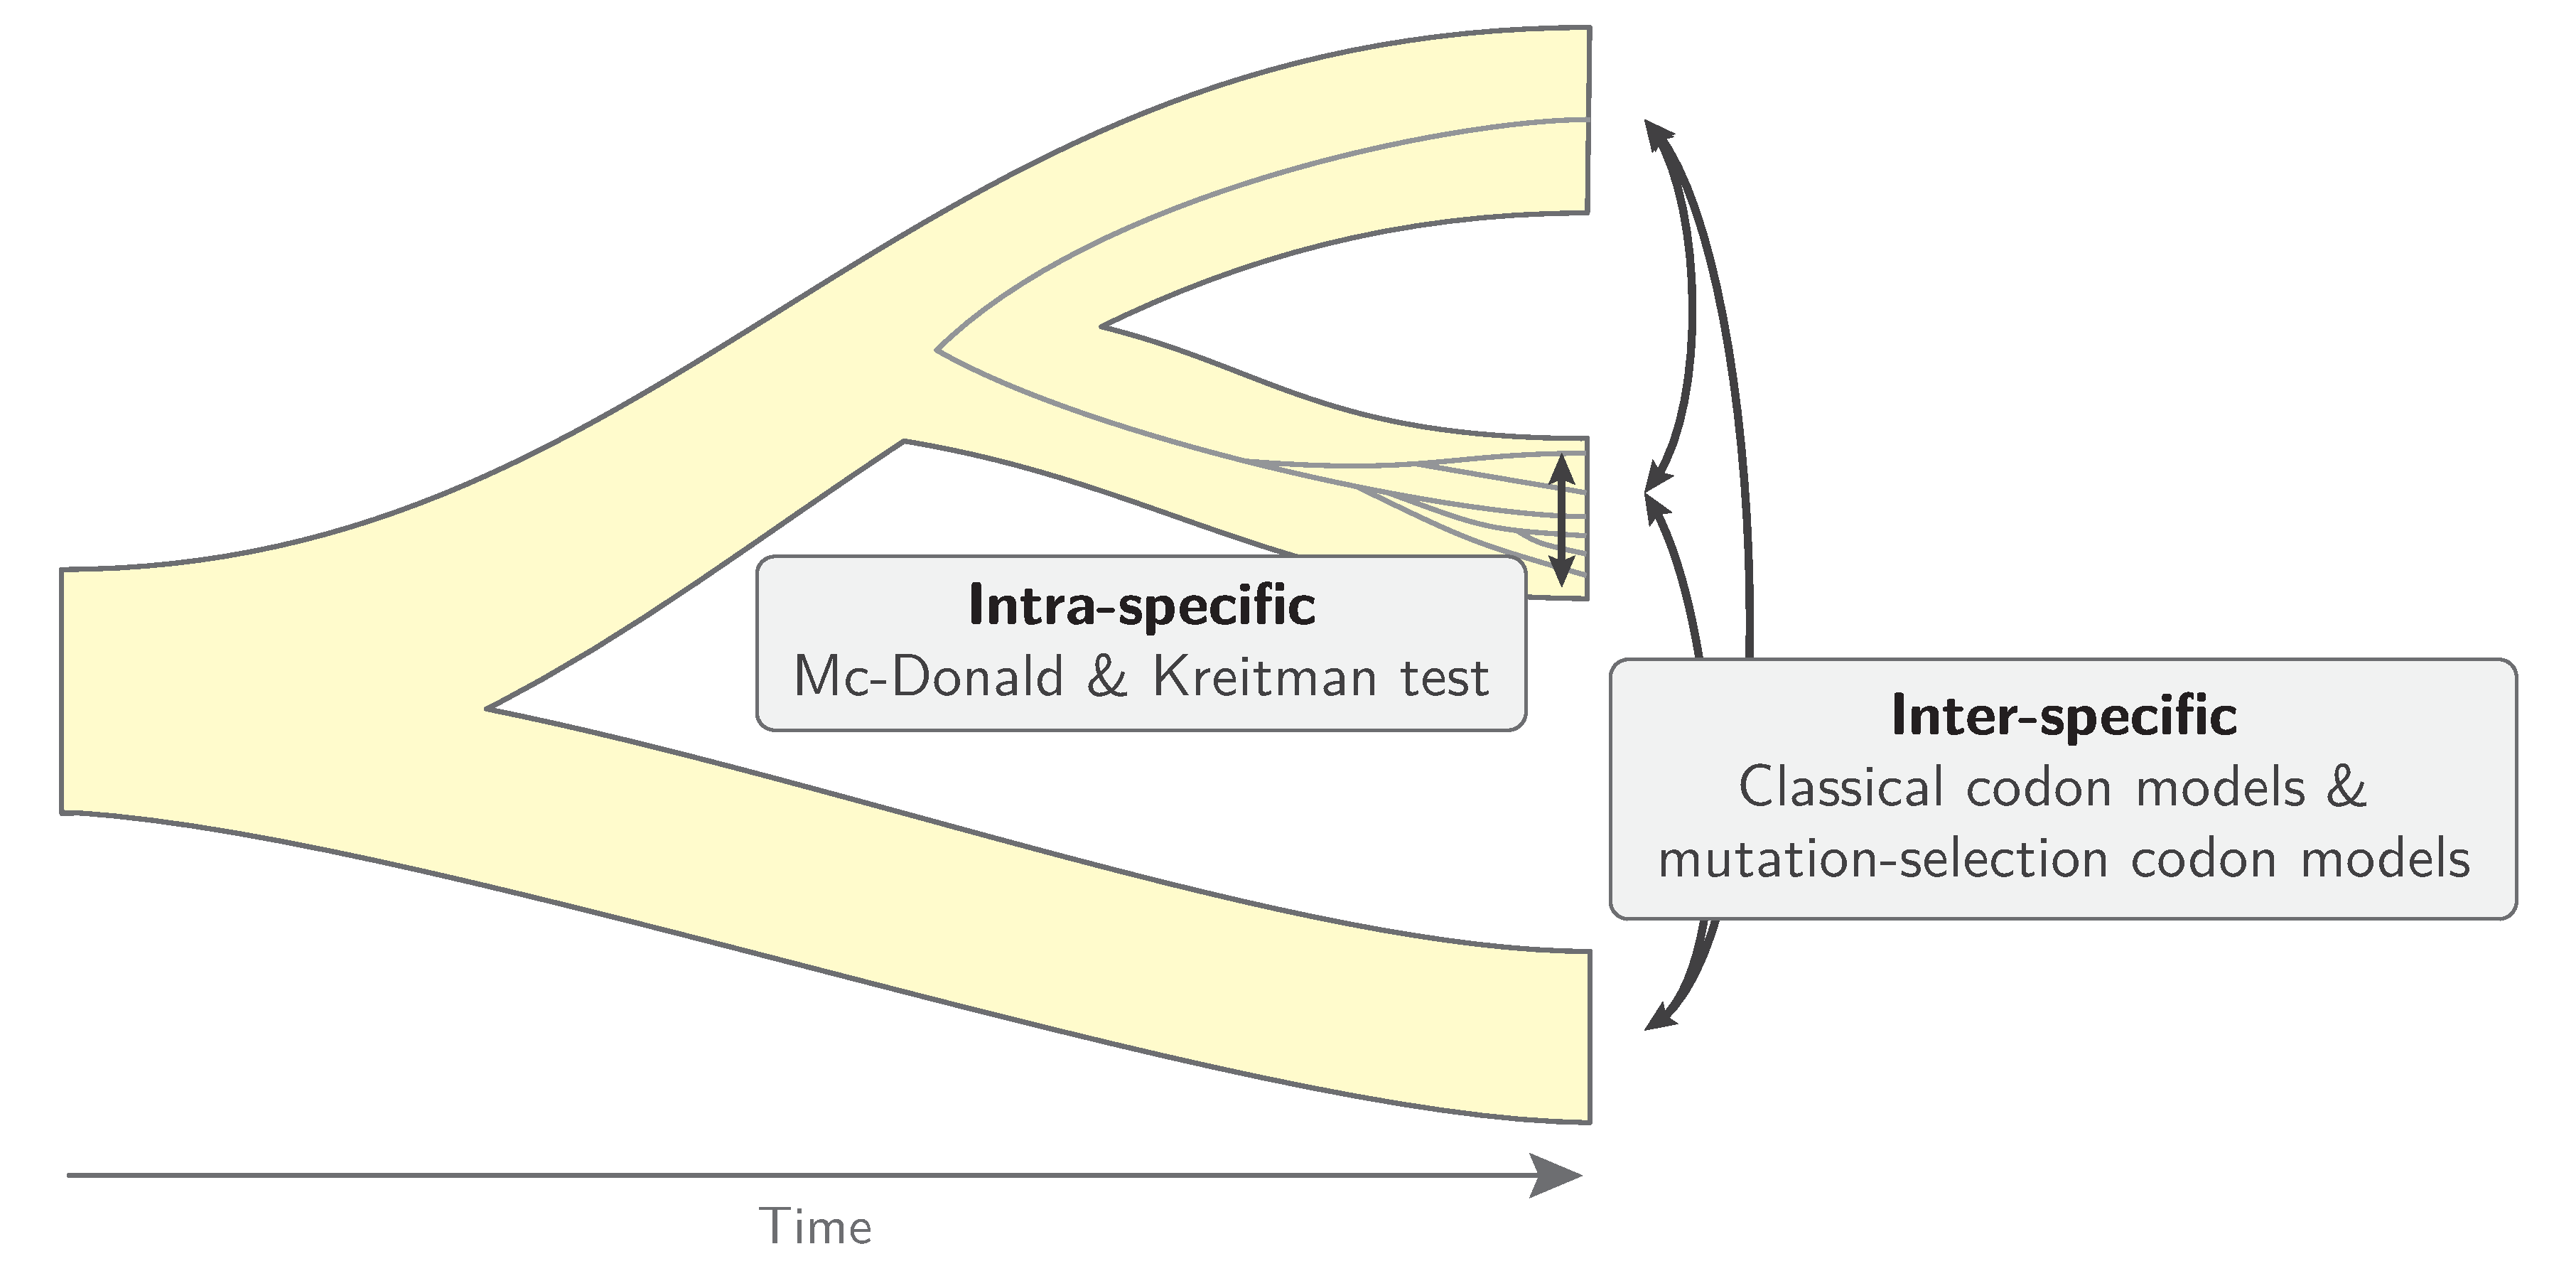
\includegraphics[width=\textwidth] {figures/inter-intra}
	\end{center}
	\caption{Detecting adaptive evolution in coding sequences from inter- and intra-specific data}
\end{figure}

The population- and phylogeny-based method work over very different time scales.
For that reason, they might be capturing different signals: isolated events of adaptation along a particular lineage for population-based method, versus long-term evolutionary Red-Queen for phylogeny based methods. On the other hand, the two signals might be correlated. This represent a unique opportunity to confound these two types of approaches on non-overlapping data frames. Accordingly, the goal of this study is to set-up a pipeline for gathering divergence and polymorphism data for coding genes across species. As a proof of concept, I analyzed 1,355 protein-coding sequences (CDS) orthologs in mammals, and conducted two separate analysis on these CDS. First, alignments in placentals (except \textit{Homo sapiens} and \textit{Pan troglodytes}) were used to run classical site-models and mutation-selection models. The method estimated the rate of adaptation in each CDS, and extracted CDS with a rate of adaptation significantly high. Secondly, the population-based method was conducted using polymorphism available in \textit{Homo sapiens} and divergence to \textit{Pan troglodytes}. The pipeline then testes if the group of sequences detected with a high rate of adaption in the phylogeny-based method also display a high rate of adaptation in the population-based method.

Finally, I investigated whether the phylogeny-based and the population-based methods give congruent results in terms of detection of adaptive evolution. 
To do so, $\omega_A^{MK}$ was computed on the concatenate of the $27$ candidates CDS inferred, by the phylogeny-based method, to have a high rate of adaptation. The result was compared to the empirical distribution of $\omega_A^{MK}$ over random sets of $27$ CDS (see figure \ref{fig:omega_snp}, panel A).
The average rate of adaptation over the $27$ candidates, such as estimated by Mc-Donald and Kreitman (see methods), is higher than the average rate of adaptation over random samples. However, the deviation is not significant ($p_{\mathrm{value}}=0.119$).\\

Similarly, using the site-frequency spectra of SNPs, $\omega_A^{DFEM}$ was computed in the same set of candidates by concatenating the $27$ site-frequency-spectrum (see figure \ref{fig:omega_snp}, panel C). And compared it to the empirical null distribution of $\omega_A^{DFEM}$ over random sets of $27$ CDS (see figure \ref{fig:omega_snp}, panel D).
The average rate of adaptation over the $27$ candidates, such as estimated using the GammaExpo model (see methods), is higher than the average rate of adaptation over random samples. In this case, the deviation is marginally significant ($p_{\mathrm{value}}=0.036$), 
meaning that modeling change in population size and the distribution of fitness effects of mutations leads to more congruence between phylogeny- and population-based methods, suggesting that the two methods are at least partially congruent in their detection of adaptation.

This study is the first medium-scale application of the phylogenetic mutation-selection method for detecting adaptation. The approach required some changes compared to the original method. More specifically, a two-step procedure was derived and deemed more reliable than the one-step \citet{lartillot_phylobayes_2013}. This approach seems to give sensible results. Its application on mammalian CDS suggests that most proteins are under \textit{nearly-neutral} regime and a few candidate proteins are under strong adaptation. The protein under adaptation also showed significant increase in ontology terms related to immune processes. In practice, there could be some background adaption in proteins categorized here as being in a \textit{nearly-neutral} regime, which might not have been detected due to lack of power of the statistical test. Further work is also needed to compare with classical codon models. Here, $27$ CDS were detected out of $1,355$. In Kosiol \textit{et al} \citet{kosiol_patterns_2008}, $400$ CDS were detected out of $16,529$ using codon site-model, suggesting that the mutation-selection model has somewhat a lower, although comparable, sensitivity compared to site-model. Ultimately, I should first scale-up the analysis to the whole dataset of $11,256$ CDS, instead of the $1,355$ CDS used because of time and computation constrains. Indeed, phylogeny-based method is computationally intensive, and requires a well resolved species tree, hence the limitation to mammals in this study. Moreover it crucially depends on the quality of the alignments, as was observed in preliminary study, and paralogs identified as orthologs or alignment problems can easily falsify the results.\\

A second objective of this work was to confront phylogeny-based and population-based methods. One main novelty of mutation-selection model, compared to classical codon models, is to provide an estimate of $\omega_A$, thus directly comparable with population-based methods. Ideally, one would like to make a quantitative comparison of $\omega_A$ and $\omega_A^{MK}$, across sequence or groups of sequences. However, the method lacked of power for two reasons. Firstly, the method did not detected enough CDS under adaptation ($27$ CDS with $\omega_A > 0$). Secondly the population-based estimation was very noisy, also requires concatenating many sequences. Nevertheless, these preliminary results are encouraging. Practically, it is possible to apply this pipeline to other species than \textit{Homo sapiens}, where polymorphic diversity is greater such as \textit{Mus} (using the same mammalian phylogeny) or \textit{Drosophila} (with another phylogeny). \\

The set of CDS detected to be under adaptation in phylogeny-based methods showed a marginally significant increase in the rate of adaption, such as inferred by population-based method. This relatively weak correlation might just reflect the limited number of CDS analyzed and the limited statistical power of the population-based method mentioned above. However, it is also possible that the two methods are inherently testing for different patterns of adaptation, meaning that recent episode of adaptation in the \textit{Hominini} lineages do not reflect the long-term patterns of adaptation. Especially since the purifying process is stronger on longer timescale, the frontier between neutral and mildly deleterious mutation is blurred on short timescale \citet{ho_time_2005}. \\

Altogether, this preliminary study suggest that the integration between population and phylogeny-based methods raises theoretical and practical issues. I suggest that further investigating these methodological integration will provide biological understanding of the evolutionary constrain of protein-coding sequences. \\


\section{Complexity}

\subsection{Epistasis}

Yet another classification of epistasis, which is helpful in the context of protein evolution,
is specific epistasis and non-specific epistasis (56) (Figure 1). Specific epistasis is structural in origin and results from direct physical interaction of spatially close residues in a protein’s 3D structure. Mutations occurring at spatially proximate sites will have non-additive contributions to the biophysical properties of proteins such as stability, activity, dynamics, or binding with partner proteins (57). Specific epistasis may also arise through long-range allosteric effects of mutations that are spatially far apart as in the case of O2 affinity in mammalian and avian Hemoglobin(40; 34). If the biophysical properties determine organismal fitness, as recently shown in examples of viral and bacterial evolution (28; 8), the non-additivity at the level of proteins translates to non- additivity at the level of fitness. As a consequence, the rate and patterns of substitution in one site may be correlated with that of another spatially close site (58; 39; 36; 46; 19).

On the other hand, non-specific epistasis arises from the non-linear dependence of
cellular/organismal fitness to biophysical properties such as folding stability (Figure 1). Even if biophysical properties are additive, the non-linear mapping of the biophysical property to fitness introduces non-linear interactions among mutations at the fitness level. Since Darwinian selection acts at the level of organismal fitness, non-specific epistasis could also affect the rate of evolution. The simplest mapping between fitness and protein properties exhibits a singlepeak, such as shown in Figure 1 for folding stability. This plateau-like fitness landscape has also been shown for the relationship between fitness and the intracellular abundance of a gene (5), between fitness and enzyme activity (26; 23; 48), and between fitness and folding stability[33]. In these simple landscapes, non-specific epistasis gives rise to the “law of diminishing returns”, i.e., the selective advantage of mutations decreases as the fitness of the organism increases, a well-known feature of many optimization processes and in adaptive trajectories in protein evolution (31; 14; 38).

\textbf{Estimating the contribution of folding stability to nonspecific epistasis in protein evolution }
The extent of nonadditive interaction among mutations or epistasis reflects the ruggedness of the fitness landscape, the mapping of genotype to reproductive fitness. In protein evolution, there is strong support for the importance and prevalence of epistasis but the quantitative and relative contribution of various factors to epistasis are poorly known. Here, we determine the contribution of selection for folding stability to epistasis in protein evolution. By combining theoretical estimates of the rates of molecular evolution and the nonlinear mapping between protein folding thermodynamics and fitness, we show that the simple selection for folding stability imposes at least ~30\% to ~40\% epistasis in long-term protein evolution. Estimating the contribution of governing factors in molecular evolution such as protein folding stability to epistasis will provide a better understanding of epistasis that could improve methods in molecular evolution.
 \citet{Dasmeh2018}


Building upon this computational convenience, complex models that allow for lineage-specific rate shifts have been developed to phenomenologically (nonmechanistically) treat signal that may originate from site-interdependence.
Gaucher EA, Gu X, Miyamoto MM, Benner SA (2002) Predicting functional divergence in protein evolution by site-specific rate shifts. Trends Biochem Sci 27: 315–321.
Whelan S, Blackburne BP, Spencer M (2011) Phyloge- netic substitution models for detecting heterotachy during plastid evolution. Mol Biol Evol 28:449–458.


Models of protein evolution that incorporate pro-
tein structure have been shown to fit data better than the corresponding models that ignore protein structure. However, an even better fit to the data could be achieved with state-of-the-art site-inde- pendent codon models.42 Despite their having pa- rameters with biologically meaningful explanations, the lackluster statistical fit of dependent site models is clearly disappointing.
41. Rodrigue N, Philippe H, Lartillot N (2006) Assessing site-interdependent phylogenetic models of sequence evolution. Mol Biol Evol 23:1762–1775.
42. Rodrigue N, Kleinman CL, Philippe H, Lartillot N (2009) Computational methods for evaluating phyloge- netic models of coding sequence evolution with de- pendence between codons. Mol Biol Evol 26: 1663–1676

Previous studies have argued that models of molecular evolution should consider the importance epistasis for its role in speciation, in modulating the rate of adaptation, and many other factors \citet{Goldstein2017, Miller2018}.
We argue that epistasis also has an important role in the response of $\omega$ to changes in $\Ne$, both in terms of susceptibility and dynamic of the response.
Fundamentally, we argue that any model modeling fitness at the site level (without epistasis) implies a slow dynamic and a strong susceptibility, and adding epistasis to the model imply a faster dynamic and a weaker susceptibility.
Intuitively, this effect originates in the fact that each site is to adapt independently to changes in $\Ne$ leading to overall a slow response (substitutions must affect all sites), and a strong susceptibility since each site will change its position in the fitness landscape.
Taking into account epistasis, the burden of adapting to changes in $\Ne$ is shared by more sites, such that all of them don't have to adapt. 
From a modeling and inference perspective, accounting for epistasis is challenging both in terms of parametrization and computational complexity \citet{Rodrigue2005, Manhart2014}. 

\subsection{$\omega_A$}


\section{Reproducible science}
I believe analytical models, computational simulations and inference models are complementary, but more importantly they are necessary to each others. 
Theoretical modeling allow to understand the principles, simulations allow to verify the soundness.
Inference allow to extract and test the theoretical results using empirical data.
Simulations have a dual role, testing the robustness of both inference procedures and theoretical results, outside of their comfort zone and assumptions.
However, this assume we are confident enough to write reproducible computations, as such the next section is dedicated to my experience and take away.

\subsection{Reproducible computations}
First, I stand firmly on the ground that data, codes and scripts should be rendered open-access of any published and peer reviewed paper.
Practically, the availability of the data and source code should simply be enforced upon submission to journal, which is currently not the case for many, even in bio-informatics and genomics fields.
This strong stance is not as to make scientist publish less, though it is a positive side-effect such as to be able to keep up with the literature.
On the contrary, is to avoid the bloating of what is called a technical debt, or research debt.
It encourages peer collaboration, both helping the team or person whom made the code available, and the community as a whole.
A straightforward way is to provide a git repository with the advantage that collaboration is facilitated trough web hosted repository such as GitLab or GitHub.

Test reproducing the results should also be made available, many tools are available to this aim \citet{Wilson2014,Darriba2018}.
When only python code is necessary for the reproductibility, anaconda/conda provides a straightforward environment to configure the necessary libraries with their versions. 
Jupyter notebooks also provide a 
For more complex environment, requiring compiling source code a more general environment is either a Docker or Singularity for example, but any containers implementing system-level virtualization is very helpful.
These tools are emerging in the community.


Workflow management system (Nexflow, Snakemake, etc) allowing to create reproducible and scalable data analyses.
Peer-coding sessions, continuous integration pipeline are valuable to use to increase the reliability of code generation.
 
\subsection{Bayesian statistics}
Knowing that maximum likelihood and Bayesian statistics are often opposed to each others and fiercely defended by their tenant I would gladly give my opinion on the matter, since I made the . 
Bayesian statistics seems personally a more comfortable inference framework than maximum likelihood for several reasons. 
First you do not need to care for local optimum which might freeze the program.
Second and most importantly, it gives the confidence interval, meaning how much certainty is available given the data on a estimate.
A corollary is that over parametrization is not an issue. 
Lasso or penalized-likelihood methods are not required.
The subjective arbitrary introduced by lasso and penalized-likelihood is replaced by statistical prior distribution, which are more meaningful.
Moreover, it gives a simple, thought extensive method to test for the repeatability and soundness of the code (cf prior distribution must match the rank).
Finally, the sampling method of 


    \chapter{Discussion \& perspectives}
\label{ch:discussion-perspectives}
{\hypersetup{linkcolor=GREYDARK}\minitoc}

As a legacy of the nearly-neutral theory, the evolution of molecular sequences is seen as a stochastic process.
One component of this process is creating diversity through mutation, while another antagonistic component is filtering out this diversity through selection, and finally the balance between these components is arbitrated by drift.
In the long term, this stochastic process results in a history of substitution events along species trees, inducing complex patterns of molecular divergence between species.
By analysing them, phylogenetic codon models aim at capturing the intrinsic parameters of evolution.

The focus of this thesis has been the development of new phylogenetic codon models and the modelling of the interplay between mutation, selection and drift in the evolutionary processes followed by protein-coding DNA sequences.
In this conclusive chapter, I first recall the main results of this thesis in section~\ref{sec:summary-of-main-results}.
Subsequently, I attempt to discuss the limitations of my work.
One main limitation concerns the problem of modelling site interdependence, which is discussed in section~\ref{sec:epistasis-and-entrenchment}.
Secondly, in section~\ref{sec:adaptative-landscape}, I draw some important connections between the mechanistic models developed here and the problem of detecting adaptive evolutionary regimes.
As a perspective, I discuss how phylogenetic mechanistic models could be unified with population genetics in section~\ref{sec:mechanistic-and-phenomenological-models}, and the inference methodology that would be adapted to such an endeavour in section~\ref{sec:mechanistic-and-phenomenological-models}.
Finally, before concluding, I discuss the question and the issue of reproducible sciences in evolutionary biology in section~\ref{sec:reproducible-science}.


\section{Summary of main results}
\label{sec:summary-of-main-results}

In chapter~\ref{chap:NucleotideBias}, I developed a phenomenological codon model in which $\omega$ is seen not as a single parameter but as a tensor (95 free parameters).
This sensor captures the small differences in fixation rate (or $\omega$) in different directions, which gives an accurate representation of how mutation and selection oppose each other at equilibrium.
This parameterization is the simplest one, in a phenomenological context, capable of correctly teasing apart mutation and selection.
Thanks to this, this modelling approach yields a reliable estimate of the mutational process, while disentangling fixation probabilities in different directions.

In chapter~\ref{chap:MutSelDrift}, I developed an extended mechanistic mutation-selection model reconstructing site-specific fitness landscape, long-term trends in effective population size and in the mutation rate along the phylogeny, from an alignment of \acrshort{DNA} coding sequences.
Simultaneously, the approach estimates the correlation between life-history traits, mutation rate and effective population size, intrinsically accounting for phylogenetic inertia.
Our framework was tested against simulated data and then applied to empirical data in mammals, isopods, primates and drosophila.
Simulated and empirical evidence suggest that there is a persistent signal in substitution patterns that relates to past history of $\Ne$, whose trends correspond to expected direction of correlation with life-history traits or ecological variables.
However, the magnitude of inferred variation in $\Ne$ across the phylogeny is narrower than expected, which is probably a bias of the approach caused by the assumptions made on the structure of the fitness landscape.

As a way to further investigate this last question, the third manuscript in chapter~\ref{chap:GenoPhenoFit} revisits the question of how the exact structure of the fitness landscape determines the quantitative response of the molecular evolutionary process, and in particular of $\dnds$, to changes in $\Ne$ and in protein expression level.
Specifically, I derive a theoretical approximation for the quantitative response of $\dnds$ to changes in both $\Ne$ and expression level, under an explicit genotype-phenotype-fitness map.
The development is generally valid for an additive trait under a log-concave fitness function, but was applied more specifically to a biophysical model in which proteins are under directional selection for maximizing their conformational stability.
In this specific case, I predict a weak response of $\dnds$ to changes in either $\Ne$ or expression level (which are interchangeable), a result corroborated by simulations under more complex models.
Based on this, I propose that fitness based on conformational stability might not provide a sufficient mechanism to explain the amplitude of the variation in the mean fixation probability which is observed empirically.
Other aspects of protein biophysics could be explored such as protein-protein interactions, which could lead to a stronger response of the mean fixation probability to changes in $\Ne$.

More globally, there is a remaining gap between quantitative predictions of biophysical models and empirical observations relating the response of protein coding sequence evolution to changes in $\Ne$ and expression level.


\section{Site interdependence and epistasis}
\label{sec:epistasis-and-entrenchment}

One of the blind spots of the mechanistic codon model developed in chapter~\ref{chap:MutSelDrift}, and more generally of current mechanistic models of the Halpern-Bruno family (see section~\ref{subsec:HB-formalism}), is the assumption of site independence.
This assumption is convenient, both computationally and statistically.
Computationally, each site can be considered as an independent Markov process (see sections~\ref{subsec:mutation-limited-assumption} and~\ref{sec-intro:likelihood}).
Statistically, one can rely on mixture models to estimate site-specific amino-acid fitness profiles (see section~\ref{subsec:empirical-calibration-HB})
In contrast, from a modelling and inference perspective, accounting for epistasis is challenging both in terms of parametrization and in terms of computational complexity (see section~\ref{subsec:structurally-constrained-site-interdependent-codon-models})
This complexity is the main reason why epistasis is generally ignored in phylogenetic models, and more particularly in codon models.
Empirically, however, evolutionary biologists have many reasons to believe that this hypothesis of site independence is not adequate, especially given our knowledge about protein biophysics (see section~\ref{subsec:conformational-stability-and-epistatis}).
This approximation is therefore problematic, and raises multiple questions.
What are the consequences of ignoring epistasis in the context of phylogenetic inference?
Practically, how could we ultimately account for epistasis in the context of inference?

Previous studies have argued that models of molecular evolution should consider the importance of epistasis for its different roles: from the importance in speciation, in modulating the rate of adaptation, in interlocking between sites (Stokes shift), downward impact on the $\dnds$ predicted by the mutation-selection models, and many other factors \citet{Goldstein2017, Miller2018}.
Based on our analysis presented in chapter~\ref{chap:GenoPhenoFit}, we argue that epistasis also has an important role in the response of $\dnds$ to changes in $\Ne$, both in terms of its susceptibility and dynamic of the response.
This is a conceptual point that, to your knowledge, had never been really identified until now.

More precisely, one key result of chapter~\ref{chap:GenoPhenoFit} is that any model without (or ignoring) epistasis implies a slow dynamic and a strong sensitivity of the mean fixation probability to changes in $\Ne$.
Intuitively, model without epistasis exhibit a slow return to equilibrium upon a change in $\Ne$ due to the waiting time until the next substitution.
Indeed, the evolutionary process is mainly mutation limited (see section~\ref{subsec:molecular-evolution-is-mutation-limited})
In addition, the mutation rate per site is very low, from $10^{-8}$ to $10^{-9}$ in mammals.
As a result, for each site, the expected waiting time until the next mutation is between $100$ to $1000$ million years, .
As for the strong sensitivity of the mean fixation probability to changes in $\Ne$, it originates in the fact that after a change in $\Ne$, each site of the sequence has to adapt independently, and change its position in the fitness landscape.

In contrast, in the presence of epistasis, the burden of adapting to changes in $\Ne$ is shared by more sites, such that not all of them (and possibly, very few of them) have to switch their position in the fitness landscape, in order for the trait to return to equilibrium under the new $\Ne$.
As a result, adding epistasis to the model implies a faster dynamic and a weaker response of the mean fixation probability to changes in $\Ne$.

These observations have several implications for empirical analyses.
First, if epistasis implies a weak response of the $\dnds$ to changes in $\Ne$, such as observed in chapter~\ref{chap:GenoPhenoFit}, for similar reasons, it may also explain the low magnitude of $\Ne$ variation estimated with site-specific mechanistic codon models in chapter~\ref{chap:MutSelDrift}.
Empirically, it appears that the susceptibility of $\dnds$ to changes in $\Ne$ is between these two extremes, namely that of site-specific fitness landscapes, and the other extreme of a single univariate phenotype controlled by all sites.
More probably, the ternary relation from sequence to phenotype to fitness implies several sites, but not all sites of the sequences, in a given phenotypic trait.

Second, the very long slow dynamic time constants implied by site-specific models are of the order of the depth of phylogeny ($100$ to $1000$ My).
As such, in the absence of epistasis, we shouldn't even see $\dnds$ correlations with either \acrshort{LHT} or $\Ne$ because of it.
Conversely, the fact that we see it is in itself an important indication of the presence of epistasis.

Ultimately, accounting for epistasis in mechanistic models of evolutions is necessary but challenging from a computational and statistical perspective.
Paths for statistical methods that can account for it are developed in section~\ref{sec:mechanistic-and-phenomenological-models}.

\section{Adaptive landscape and positive selection}
\label{sec:adaptative-landscape}

Another blind spot the mechanistic phylogenetic codon model developed in chapter~\ref{chap:MutSelDrift} is the absence of adaptive evolution (see section~\ref{subsec:where-is-adaptation?}).
Indeed, the mutation-selection equilibrium is essentially a nearly-neutral regime.
As a result, at mutation-selection equilibrium, the sequence is close to the fitness optimum and therefore, most mutations are deleterious or compensate for previous deleterious mutations that reached fixation.
Adaptation, on the other hand, can be seen as a process where the underlying fitness landscape is not fixed (i.e. time-independent) but is instead dynamic (i.e. time-dependent).
In other words, it is not so much a fitness landscape than fitness seascapes~\citep{Mustonen2009}.
Under a fitness seascape, the sequence is constantly running after a moving target, and as a result, there is net flux of adaptive substitutions (see section~\ref{subsec:adaptive-evolution}).

\subsection{Mechanistic mutation-selection models under fitness seascapes}
\label{subsec:mechanistic-fluctuating-selection}

In the context of a mutation-selection framework, explicitly modelling adaptation in terms of fitness seascapes fluctuating along the phylogeny appears to be challenging.
A first direction is to consider that adaptation consists in changes in the site-specific fitness profiles along some lineages.
These changes can either be informed by experimental mutational scanning~\citep{Bloom2017}, or estimated using a priori knowledge of phenotypic changes or ecological shifts\citep{Tamuri2009, Parto2018, Parto2018a}.
Without knowledge of the drivers of adaptation, modulations of the fitness profiles through time could also be implemented as a Markov modulated process along the phylogeny.
However, such an endeavour would be statistically and computationally challenging and might require to first rethink the entire statistical approach (see section~\ref{sec:mechanistic-and-phenomenological-models}).

\subsection{Hybrid mechanistic and phenomenological mutation-selection models}
\label{subsec:hybrid-mechanistic-and-phenomenological-mutation-selection-models}

As an alternative to explicit models of adaptation through fitness seascapes, the current nearly-neutral mutation-selection framework can be leveraged as a null model.
Deviation from this null model can be seen as a signal of adaptation (see section~\ref{subsec:adaptive-evolution}).
In particular, if the sequences are under recurrent positive selection, the mean fixation probability ($\avgpfix$) of non-synonymous mutations will tend to be higher than predicted by the purely nearly-neutral model.
This discrepancy between the mean fixation probability and the nearly-neutral expectation can be captured by a deviation parameter $\omega_*$, as in \citet{Rodrigue2016}.

Thus far, however, this idea has been implemented only at the gene level (i.e. invoking a single $\omega_*$ for the whole gene).
Yet, adaptation often occurs more locally, in specific domains of the protein.
Accordingly, this gene-wide deviation parameter $\omega_*$ could be refined at the site-level.
In this direction, in a work led by Nicolas Rodrigue, we developed a method to detect site-specific adaptation as a deviation from a null nearly-neutral model of evolution.
This method has been developed in the generic programming environment provided by \texttt{BayesCode} (see section~\ref{subsec:implementation}), and the manuscript accepted in the journal \textit{Molecular Biology \& Evolution} is available in appendix page~\pageref{sec-appendix:MutSelM3starMBE}.
These methods are relatively new, and must still be validated, more broadly applied to empirical data, and their predictions more extensively compared with those obtained from with classical codon models.

However, in its current form, phylogenetic model seeking adaptation as a deviation from near-neutrality assumes a constant $\Ne$ across the tree.
As already discussed, this assumption is of course not reasonable.
A simple solution to this problem would be to add a deviation parameter $\omega_*$ in the mechanistic model developed in chapter~\ref{chap:MutSelDrift}.
The resulting model would potentially be more effective at detecting positive selection.

Interestingly, $\omega_*$ could also be allowed to vary across branches, like $\Ne$.
This could have useful applications.
For instance, bats are known to be reservoirs of pathogens.
Recent results suggest they have more efficient immune system~\citep{Baker2013,Pavlovich2018}, such that proteins involved in host-pathogen interactions are under positive selection~\citep{Hawkins2019,Vandewege2020}.
But also, bats have large population sizes, compared to other mammals, and thus more efficient purifying selection.
These two factors have opposing effects on $\dnds$, and teasing them out might therefore be difficult using classical codon models.
In contrast, the mutation-selection model with both $\Ne$ and $\omega_*$ varying across lineages could offer a way to estimate them separately, which would allow to address the problems mentioned above.
Thus, do bats, compared to other mammals, have both stronger purifying selection (lower $\dnds$) due to large $\Ne$ and stronger positive selection (larger $\omega_*$)?

\subsection{Detecting adaptation with polymorphism}
\label{subsec:detecting-adaptation-with-polymorphism}

Phylogenetic codon models are only one of the methods currently available to detect adaptation.
There are other approaches that are widely used in population genetics, and that make use of the signal contained in polymorphism data, such as originally pioneered by \citet{McDonald1991}.
The idea behind the McDonald \& Kreitman (\acrshort{MK}) approach is to decompose the rate of selected substitutions ($\omega_{\text{Tot}}$), as a mixture of both advantageous substitutions and non-adaptive (nearly-neutral) substitutions:
\begin{align}
    \omega_{\text{Tot}} & = \omega_{\text{A}} + \omega_{\text{NA}}, \\
    \iff \omega_{\text{A}} & = \omega_{\text{Tot}} - \omega_{\text{NA}},
\end{align}
where $\omega_{\text{NA}}$ is the rate of substitution contributed by non-adaptive nearly-neutral evolution and $\omega_{\text{A}}$ is the total rate of substitution contributed by adaptive evolution.
In this context, under the assumption that adaptive mutations are rare, the ratio of non-synonymous over synonymous polymorphism ($\pnps$) mostly contains non-adaptive polymorphism and is a measure of $\omega_{\text{NA}}$:
\begin{equation}
    \omega_{\text{NA}} \simeq \pnps.
\end{equation}
Moreover, the total rate ratio of non-synonymous over synonymous substitutions ($\dnds$), estimated from divergence data, is a measure of $\omega_{\text{Tot}}$:
\begin{equation}
    \omega_{\text{Tot}} \simeq \dnds.
\end{equation}
Altogether, the rate of adaptive evolution, which contributes disproportionately to the divergence are estimated as the difference between divergence and polymorphism:
\begin{equation}
    \omega_{\text{A}} \simeq \dnds - \pnps.
\end{equation}

However, estimation of the non-adaptive rate through $\pnps$ can be biased by moderately deleterious mutations and by the change in population size through time~\citep{eyre-walker_changing_2002}.
To overcome these biases, a method initially proposed by \citet{eyre-walker_estimating_2009, Galtier2016} relies on the synonymous and non-synonymous site-frequency spectra (\acrshort{SFS}) to correct for demography and to estimate the distribution of fitness effects of mutations (\acrshort{DFE}), modelled as a continuous distribution.
This method, and subsequent developments which are reviewed in \citet{Moutinho2019a}, provide more reliable estimates of $\omega_{\text{NA}}$ and, as a result, a better estimate of $\omega_{\text{A}}$.

\subsection{Confronting methods for detecting adaptation}
\label{subsec:confronting-methods-for-detecting-adaptation}

The availability of independent phylogenetic methods (based on either phenomenological and mechanistic codon models) and population genetics approaches (using the McDonald \& Kreitman ideas) for detecting adaptation raises the question whether they detect congruent signals of adaptation.

Empirically, phenomenological and mechanistic codon methods should be confronted to McDonald \& Kreitman (\acrshort{MK}) methods.
In the case of the overlap between positively selected genes detected with phenomenological codon models and with \acrshort{MK} methods, the set of genes detected does not seem to overlap beyond random expectation~\citep{He2020}.
In contrast, at the site level, classical codon models are congruent with \acrshort{MK} methods, with most adaptive mutations occurring at the surface of proteins in both methods~\citep{Moutinho2019}.
These results still need be refined across clades and genes, and the availability of polymorphism and divergence \acrshort{DNA} sequences that are aligned will make this comparison possible.

However, positively selected genes or sites detected by classical codon models and \acrshort{MK} methods can theoretically be different, since non-adaptive part of substitution ($\omega_{\text{NA}}$) is subtracted in \acrshort{MK} test while classical codon models are not accounting for it.
Interestingly, another estimate of $\omega_{\text{NA}}$ in the context of phylogenetic codon model is what was referred to as $\omega_0$ in the context of the mutation-selection null model (see section~\ref{subsec:HB-formalism-nearly-neutral-model}).
As a result, mechanistic mutation-selection codon models ($\omega_0$) and \acrshort{MK} test ($\pnps$) should theoretically be more directly comparable.
From the availability of divergence and polymorphism data, it is now possible to ask whether the rate of non-adaptive evolution measured by phylogenetic mutation-selection models and \acrshort{MK} methods are congruent, and if not the reason for such discrepancy should be understood.

\begin{figure}[htbp]
    \centering
    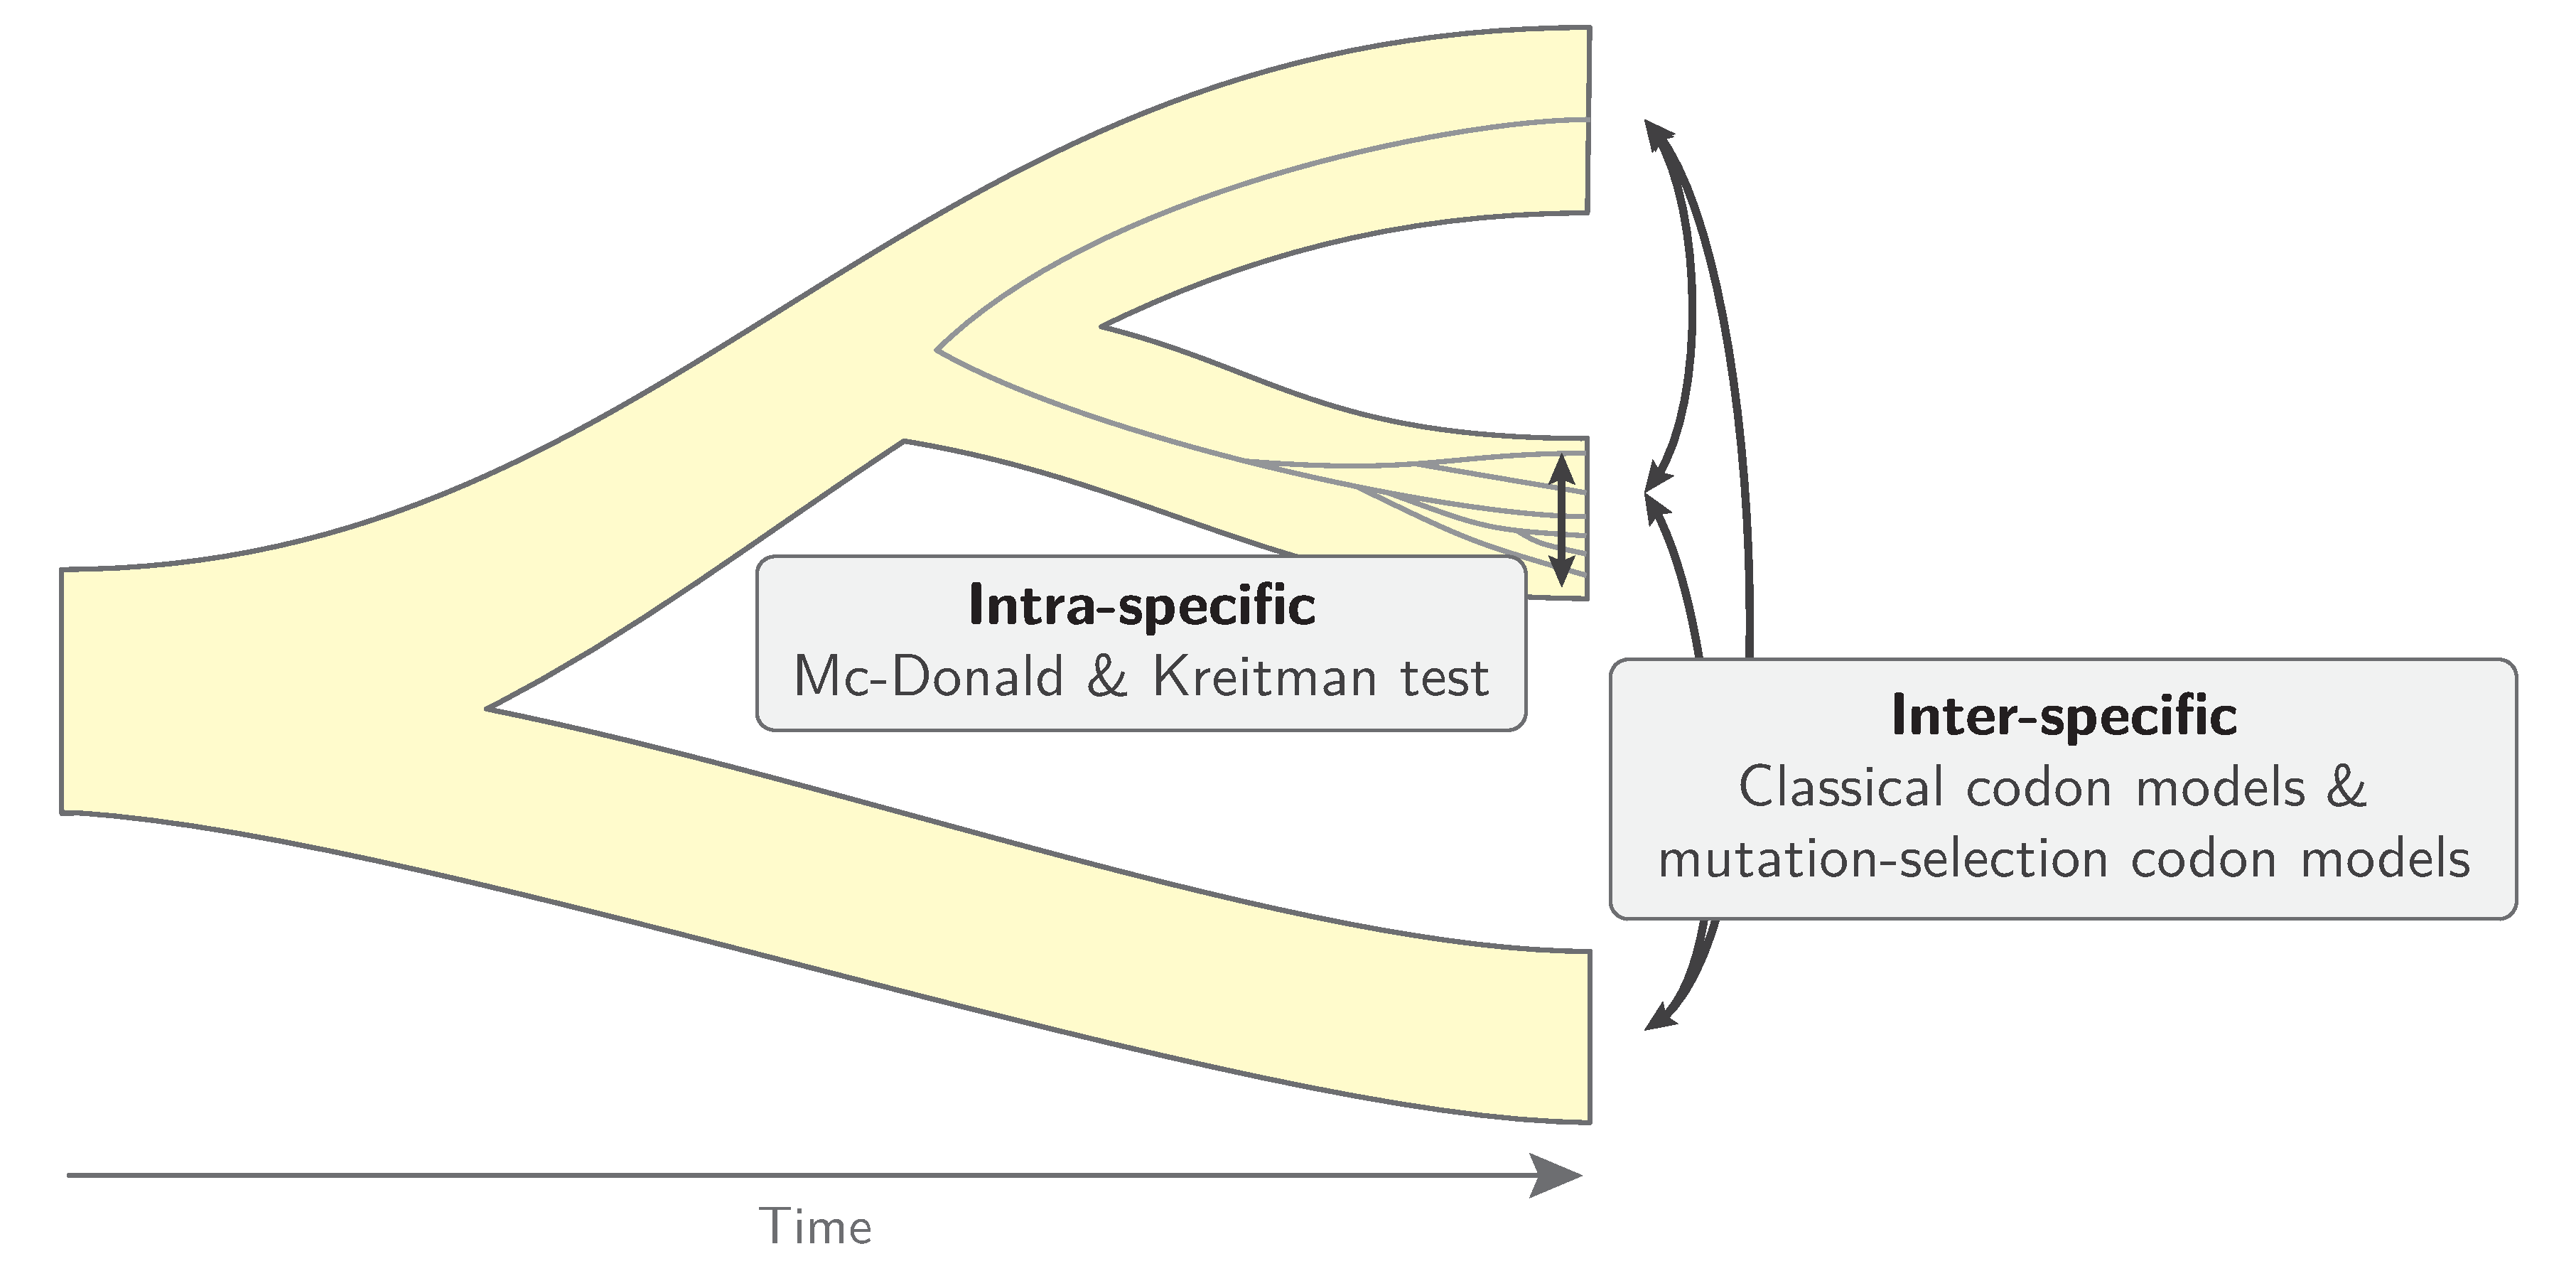
\includegraphics[width=\textwidth] {figures/inter-intra}
    \caption{Detecting adaptive evolution in coding sequences from inter- and intra-specific data}
    \label{fig:detecting-adaptation-inter-intra}
\end{figure}

\section{Unifying phylogenetic and population-genetics model}
\label{sec:unifying-phylogenetic-and-population-genetics-model}

Throughout this manuscript, the phylogenetic codon models that have been presented have so far ignored genetic diversity within species.
As a result, all differences observed in the alignment are assumed to be substitutions.
However some of the differences observed in the alignment might in fact be polymorphisms segregating in the population.
Moreover, substitutions are not instantaneous and ancestral shared polymorphisms can result in incomplete lineage sorting~\citep{Charlesworth2010}.

Mistaking polymorphisms for substitutions is problematic, since both are not sensitive to mutation, selection and drift to the same extent~\citep{Mugal2014}.
For example, the neutral diversity increases with $\Ne$, while the rate of neutral substitutions is insensitive to $\Ne$.
Also, mildly deleterious can be present in polymorphism while being filtered out by selection and not present in substitutions.

Finally, substitution rates are much more strongly influenced by selection, and more generally by fixation biases (such as gBGC) than polymorphisms, which are primarily reflecting mutation biases.

Interestingly, this suggests that polymorphism and divergence could be leveraged together to help disentangle mutation, selection and drift.
In other words, phylogenetic and population-genetic approaches could be unified, in the context of a single modelling framework~\citep{Thorne2012}.

Such an integration between phylogenetic and population genetics as already been attempted in several studies.
For example, \citet{Wilson2011} modelled codon evolution in a joint framework with $3$ species, which allowed them to analyse the variation in selection pressure spatially along the genome and temporally between lineages.
However, this methodology proved to be computationally intensive and does not scale well with the number of extant species.
Alternatively, modelling substitutions as mutational events followed by a gradual fixation, using an explicit Wright-Fisher or Moran process along the phylogeny, makes it possible to estimate nucleotide mutation rates and mean fixation probabilities from genetic variation within and between species, while accounting for shared ancestral polymorphisms and incomplete lineage sorting~\citep{DeMaio2013, Schrempf2016, Bergman2018, Schrempf2019}.
In particular, this methodology was used to disentangle \acrshort{gBGC} and the mutational bias~\citep{Borges2019, Borges2020}.
However, this methodology does not scale well with the number of states of the models.
For that reason, it would be particularly difficult to translate the approach from nucleotides (4 states) to codons (61 states).

Because mechanistic codon models are based on population-genetic first principles, they can theoretically be extended to account for within species diversity.
One strategy would be to augment molecular divergence data between species with information about molecular polymorphism within species.
Such an attempt has been tried during the first year of the PhD.
The formalism that was used is based on Poisson Random fields (details can be found in appendices page~\pageref{sec-appendix:PRF}).
This extension was rather straightforward to implement in \texttt{BayesCode}, in the context of site-specific mechanistic codon models.
% This was historically the reason why I decided to extend phylogenetic site-specific mutation-selection codon models by incorporating branch-specific $\Ne$, such as presented in chapter~\ref{chap:MutSelDrift}.

A first implementation was tested against simulation under a Wright-Fisher model of evolution along the phylogeny.
It yields an accurate estimation of diversity ($\theta = 4 \Ne u$) in extant species, and is able to better tease out mutation and selection by leveraging both divergence and polymorphism signal.
However, it was found to be computationally intensive, even with the use of sufficient statistics to accelerate the computation (see section~\ref{subsec:suffstats-data-augmentation}).
Moreover, the assumption of a constant $\Ne$ along the phylogeny assumed by mutation-selection codon models was arguably the strongest assumption to relax in this context~\citep{Rousselle2018}.
Indeed, what sense would it make to integrate empirical data about genetic diversity in extant species that generally have quite different levels of diversity if $\Ne$ is considered constant along the phylogeny.
This was historically the reason why I decided to first extend phylogenetic site-specific mutation-selection codon models by incorporating branch-specific $\Ne$, such as presented in chapter~\ref{chap:MutSelDrift}.

Once incorporating branch specific $\Ne$ , the original goal was then to add polymorphism data in the context of this improved mutation-selection codon model.
As it turns out, however, there are other issues that needed to be addressed, before achieving this integration.
In particular, the fact that the range of $\Ne$ inferred by the model turns out to be too narrow (see section~\ref{chap:MutSelDrift}), as well as computational issues.
Indeed, with branch-specific $\Ne$ and extant polymorphism, the computing time to reach convergence of the \acrshort{MCMC} became prohibitive.

Retrospectively, even though site- and branch-specific mutation-selection phylogenetic codon models can be extended by incorporating empirical data about polymorphism, as I have started to do in \texttt{BayesCode}, I believe it is not yet the path forward to build a unified phylogenetic and population-genetic model.
Before doing this, I believe phylogenetic codon models and population-genetics method should first be confronted, and the discrepancy should be understood, such as presented in the previous section.
The impact of epistasis should also be better understood and characterized.
Only in a second step, subsequently to this confrontation, could phylogenetic models in principle accommodate extant polymorphism.
However, this will probably require another approach of inference, more computationally reasonable that the one that I have explored in my work (in chapter~\ref{chap:MutSelDrift}).


\section{Mechanistic and phenomenological models}
\label{sec:mechanistic-and-phenomenological-models}

% Categories of models
Models of inference are classified broadly into phenomenological and mechanistic~\citep{Rodrigue2010a}.
Mechanistic models dissect the detailed causal chain of events responsible for each substitution event and then use this to construct a detailed model from first principles.
By doing this, they relate structural, population genetics and ecological parameters to the likelihood function (see chapter~\ref{chap:MutSelDrift}).
As such, mechanistic inference models are suitable to construct an integrative framework, for example relating the signal available in molecular sequences to structural parameters, expression level across genes and varying effective population size across lineages.

Once such models have been fitted to empirical data, the estimated parameters can then be confronted with independent estimations, which allow one to robustly test the model since independent estimates of biological and ecological parameters should of course be congruent~\citep{Dasmeh2014}.
However mechanistic models are computationally very intensive, to a point where they can reach the current limits in available computing power.
Apart from this physical limit of resource available, the use of computing resources bears ecological consequences on environmental degradation and $C0_2$.
Moreover, increased complexity of the models bears another consequence: the liability of the code and software decreases, compromising the reproducibility of the results obtained with such models.
For these reasons (and primarily the computational limitations), mechanistic models tend to make a number of strong simplifying assumptions (such as no epistasis), which can have detrimental effects on the robustness of the inference (see chapter~\ref{chap:MutSelDrift}).

In contrast, phenomenological models are formulated in terms of aggregate parameters, capturing the average rate of synonymous or non-synonymous substitutions, or their ratio.
Their aim is to determine the statistical distribution of these aggregate quantities across the tree, across genes, or across sites, but without deriving them from first principles.
Compared to mechanistic models, they are computationally much more efficient.
On the other hand, they do not give direct access to the population-genetic parameters.

This raises the question of how to benefit from the advantages of the two approaches.
Observations and experiments done throughout this thesis led me to crystallize the conception that models of inference should be mechanistic in essence, in the sense that they should be parameterized by variables that are derived from first principles.
But should be phenomenological in practice, in the sense that these variables should nevertheless be aggregate parameters.

The first manuscript presented in this thesis (chapter~\ref{chap:NucleotideBias}) gives some preliminary directions to accomplish this project.
A mean-field argument was used to derive a phenomenological model based on an underlying mechanistic site-specific model.
As a result, the mean-field parameters of the phenomenological model capture aggregate quantities that are averages across sites.
The phenomenological model that was obtained using this approach is easier to fit to the data.
Nonetheless, it captures essential parameters that are easy to interpret mechanistically, after the fact.

Altogether, hybrid models based on mechanistic first principles but obtained by deriving aggregate parameters are avoiding the pitfalls of both approaches, being based on independently identifiable parameters and at the same time being computationally parsimonious.
Such hybrid models can be developed with the following procedure:
\begin{enumerate}
    \item Define a mechanistic microscopic model from molecular first principles (see chapter~\ref{chap:GenoPhenoFit}).
        This model can be potentially complex, modelling all kinds of variations, such as for example incorporating site interdependence or polymorphism within species.
        Such model is meant to be implemented in simulations, but never in inference.
    \item Use a mean-field argument and calculate aggregate quantities emerging from the microscopic model, leveraging population genetics first principles.
        Possibly, use theoretical developments such as presented in chapter~\ref{chap:GenoPhenoFit} to approximate the response of the aggregate quantities to changes in the underlying mechanistic parameters.
    \item Implement the inference phenomenological model whose parameters correspond to the mean-field aggregates.
        Such phenomenological model is meant to be confronted with simulation under the mechanistic model.
        And subsequently applied to empirical data to estimate the parameters of interest, and their covariation with variables that might change across species or across genes.
\end{enumerate}
Such endeavour, however, requires mathematical work to derive the relationship between parameters of interest (such as $\EmpiricalDeltaDeltaG, \Ne, $ expression level, \ldots) and aggregate parameters of evolution that are extractable from the data ($\avgpfix$).
Chapter~\ref{chap:GenoPhenoFit} represents one such mathematical development.

\section{Reproducible science}
\label{sec:reproducible-science}

This thesis is based on a combination of analytical developments, computational simulations and inference models, which I argue are complementary, but more importantly, they are all jointly required.
Theoretical modelling allows one to understand the principles, while simulations are crucial to verify the soundness.
Inference makes it possible to extract and test the theoretical results using empirical data, which are verified and tested against simulations.
Simulations have thus a dual role, testing the robustness of both inference procedures and theoretical results, outside of their comfort zone and assumptions.
However, this assumes we are confident enough to write reproducible programs.
In this direction, the next section is dedicated to my experience in reproducing results.

First, I stand firmly on the ground that data, codes and scripts should be rendered open access for any published and peer reviewed paper.
Practically, the availability of the data and source code should simply be enforced upon submission to journal, which is currently not the case for all journals, even the fields of bioinformatics and genomics.
It is true that such enforcement imposes a heavier burden on scientists upon publishing.
However, it avoids the bloating of the technical debt, or research debt resulting from building theories on the ground of a dangerous and possibly shaky basement.
It encourages peer collaboration, both helping the team or person(s) who made the code available, and the community as a whole.
A straightforward approach is to provide a \texttt{git} versioned repository, with the advantage that collaboration is facilitated through web hosted repositories such as \texttt{GitLab} (hosted by institutions) or \texttt{GitHub} (hosted by private company, here Microsoft).

Nonetheless, code availability is a necessary condition, but not the sole requirement of reproducible research.
Specific instructions to reproduce the results should also be made available, where many tools are available to this aim~\citep{Wilson2014,Darriba2018}.
The first step to reproduce a code is to have the required environment, meaning the necessary libraries and dependencies for the code and scripts.
For script and code written in \texttt{Python}, the package manager \texttt{Anaconda} (or \texttt{Conda}) provides a readily available environment to configure the necessary libraries with their versions.
More complex environment requiring code compilation or system-level packages can leverage containerization technology such as \texttt{Docker} or \texttt{Singularity} for example, but any other containers implementing system-level virtualization is very helpful to provide the necessary libraries.
Once the environment is specified, the documentation can be made available as a README with the necessary instructions.

More generally, notebooks such as \texttt{Jupyter Notebook}, \texttt{RMarkdown} or \texttt{Org-mode} to name a few also provide an environment knitting together code and instructions, allowing anyone to follow step-by-step experiments, analysis and results, in a similar fashion as laboratory notebook required in wet labs.
It is important to note that notebooks can run code from a variety of languages (\texttt{C++}, \texttt{Haskell}, \texttt{Java}, \texttt{Julia}, \texttt{Python}, \texttt{Wolfram Language}, \texttt{Matlab}, \texttt{Ruby}, \ldots).
These tools are emerging in the community, as well as workflow management system (\texttt{Nexflow}, \texttt{Snakemake}, \ldots) allowing one to create reproducible and scalable data analyses running on computing clusters.

Using this range of tools helps other scientists who might want to understand, test or build upon published work.
Moreover, they are also very helpful for the person or team implementing them, since a more rigorous and reproducible environment makes it possible to more easily track down bugs and test programs under different conditions or datasets\footnote{Notebooks are very useful to present work and data analysis, but should not be used during development since they often offer poor integration with debugger and code inspection tools, enforce awkward software design patterns, and often result in bloated versioned repository.}.
During the development period, continuous integration pipelines are valuable to increase the reliability of code generation, which should be used whether working alone or inside a team, but is, of course, more critical for collaborative code where one cannot control all of the code that is written.

Collaborative coding practices such as peer-coding sessions are really useful to implement critical code at the core of the program under development.
I argue that efficient peer-coding sessions can be organized by dividing the tasks into a group focused in the detailed implementation while the others are free to focus on edge cases and on the overall implications of different implementations.
Moreover, peer-coding sessions provides a convenient and structured place for learning good practices, for expanding its technical knowledge while correcting bad habits.

Another remarkable practice is to write two independent versions of the program, using if possible different algorithms and languages but with the same functionality, but most importantly, by a different person.
Then testing the programs against each other under the same conditions and datasets should result in the same outcomes\footnote{An extreme version is adversarial coding (or chaos engineering), where the goal is to find conditions on which the adversary program fails.}.
Such a model of reproducible computing experiments and analyses is laborious and demanding, but I argue this is the definition of reproducibility we collectively should aim for, namely where one can independently reproduce the same experiment.
If reproducibility fails, one can run the code with different conditions to pinpoint the failing code (which might actually be in both versions).
Personally, having practised this method, I strongly believe it pervasively reduces our research debt that we might inadvertently burden others with whenever not realizing the program is bugged, and that is also ultimately save us time on debugging and conducting research.
Finally, explaining to others our choices of algorithms, implementation and data structure forces us to express intelligibly our ideas and, therefore, to better understand them, while gaining from others insights and new algorithmic expertise.


\section{Concluding remarks}
\label{sec:concluding-remarks}

To conclude, this work is an encouraging, although still far from complete attempt to build integrated models of the evolution of protein-coding \acrshort{DNA} sequences.
I think my work contributed to consolidating the idea that the patterns of substitutions inform us on the long-term fluctuations in genetic drift along branches and selection along sequences.
This thesis also further emphasizes that the assumptions made on the structure of the fitness landscape have a critical importance on the sensitivity of changes in substitution rates to changes in ecological ($\Ne$) or molecular variables (protein expression level).
Conversely, empirical observations of the patterns of substitutions in response to changes in molecular or ecological variables inform us about the underlying structure of the fitness landscape.

Altogether, this work can be seen as a building block, toward bridging phylogeny and population genetics.
Constructing an integrated framework is theoretically possible but with a still limited scope so far.
However, confronting the estimation of phylogenetic codon models and population-genetics approaches, for example, on the question of the rate of adaptive substitution, is a path forward toward an integrated view of protein-coding DNA sequence evolution.
Finally, I believe this thesis is not providing disruptive results, but instead is consolidating theoretical models on which molecular evolution is based, and points out some of the pitfalls to avoid.

	
    % \appendix           % "Chapter" is renamed "Appendix"
    % \appendixpage       % Similar to \part*{Appendices}, but appears in TOC
    % \chapter{Discussion}

    
    \backmatter         % Folios in Arabic numerals, unnumbered chapters.
   	\bibliographystyle{natbib}
	\bibliography{references}

\end{document}